\documentclass{ufpatcc}

\include{include}
%% Packages used for the TCC

%\usepackage{booktabs}

%%%% Definitions and New commnads %%%%

\newcommand{\sen}{\operatorname{sen}}
\newcommand{\mbeq}{\overset{!}{=}}

\renewcommand\Re{\operatorname{Re}}
\renewcommand\Im{\operatorname{Im}}

%%%% New control sequences %%%%

\newcommand{\redeq}[1] {\textcolor{red}{#1}}
\newcommand{\blueeq}[1] {\textcolor{blue}{#1}}
\newcommand{\att}[1] {\textcolor{red}{#1}}
% Used Packages:
\usepackage{tikz}
\usepackage{float}
\usepackage{steinmetz}
\usetikzlibrary{arrows,shapes,shapes.multipart}
%\usepackage[brazil]{babel}
\usepackage[T1]{fontenc}
\usepackage[utf8]{inputenc}
\usepackage{amsmath}
\usepackage{amsfonts}
\usepackage{enumitem} % To adjust lists
\usepackage{verbatim} % Multi-line comments
\usepackage{mathabx} % Package that contains the circular convolution symbol
\usepackage{graphicx}
\usepackage{caption}
\usepackage{subcaption}
\usepackage{units}
\usepackage{adjustbox}
\usepackage{dirtytalk}

%\usepackage[backend=bibtex8]{biblatex}

\ifpdf

\ifdefined\hyperref
\else
\usepackage[pdftex,colorlinks]{hyperref}
\fi

\hypersetup{%
pdftitle={Some title},
pdfauthor={Your name - LaPS - UFPA},
pdfkeywords={DSP,Signal},
pdfstartview={FitH}, %% <--
urlcolor=black,
%linkcolor=blue,
linkcolor=black,
%citecolor=red,
citecolor=black,
}

% Ensiar o Latex a separar silabas
\hyphenation{DMT En-ge-nhei-ro}


\ufpaTitulo{An FPGA-Based Radio Frontend for LTE Transmission on Cloud RAN}

\ufpaAutor{Gabriel Peixoto de Carvalho}
\ufpaSegundoAutor{}
\ufpaOrientador{Prof. Aldebaro Barreto da Rocha Klautau Junior}
\ufpaCoordenadorCurso{Prof. Francisco Carlos Bentes Frey Muller}

\ufpaCoOrientador{Prof. Wilson Pacheco Ferreira}
\ufpaMembroBancaA{Prof. Francisco Carlos Bentes Frey Muller}
\ufpaMembroBancaB{Eng. Igor Mesquita de Almeida}


\begin{document}

\ufpaPaginaDeRosto

\ufpaPagRostodo

\ufpaPaginaDeAprovacao

%%%%%%%%%%%%%%%%%%%%
%   Oferecimento   %
%%%%%%%%%%%%%%%%%%%%

\begin{ufpaOferecimento}
\index{Oferecimento@Oferecimento}%
\addcontentsline{toc}{chapter}{Dedicatoria}

\end{ufpaOferecimento}

%%%%%%%%%%%%%%%%%%%%
%  Agradecimento   %
%%%%%%%%%%%%%%%%%%%%

\begin{ufpaAgradecimentos}
\index{Agradecimentos@Agradecimentos}
\addcontentsline{toc}{chapter}{Agradecimentos}

\begin{flushright}
Gabriel Peixoto de Carvalho
\end{flushright}

\end{ufpaAgradecimentos}

%%%%%%%%%%%%%%%%%%%%
%      Ep�grafe     %
%%%%%%%%%%%%%%%%%%%%

\begin{ufpaEpigrafe}
Viva como se voce fosse morrer amanha. Aprenda como se voce fosse viver para sempre.\\
\begin{flushright}Mahatma Gandhi\end{flushright}
\end{ufpaEpigrafe}

%%%%%%%%%%%%%%%%%%%%%
%  Lista de Siglas  %
%%%%%%%%%%%%%%%%%%%%%

\chapter*{List of Acronyms} \label{sec:siglas}
\begin{enumerate}
 \item ADSL - \textit{Linha de assinante digital assim�trica}
 %\item AWGN - \textit{Ru�do aditivo branco Gaussiano}
 %\item BER - \textit{Taxa de erro de bit}
 %\item DFT - \textit{Transformada de Fourier discreta}
 %\item DMT - \textit{Multi-tom discreto}
 %\item DSL - \textit{Linha de assinante digital}
 %\item FEQ - \textit{Equalizador em frequ�ncia}
 %\item FFT - \textit{Transformada rápida de Fourier}
 %\item FTTH - \textit{Fibra até a residência}
 %\item G.fast - \textit{Acesso rápido aos terminais do assinante}
 %\item ICI - \textit{Interferência inter-portadora}
 %\item IDFT - \textit{Transformada de Fourier discreta inversa}
 %\item IFFT - \textit{Transformada rápida de Fourier inversa}
 %\item ISI - \textit{Interferência inter-simbólica}
 %\item OFDM - \textit{Modulação por divisão ortogonal de frequência}
 %\item PC - \textit{Prefixo cíclico}
 %\item PSD - \textit{Densidade espectral de potência}
 %\item RIC - \textit{Resposta impulsiva do canal}
 %\item SC - \textit{Sufixo cíclico}
 %\item SER - \textit{Taxa de erro de símbolo}
 %\item SNR - \textit{Razão sinal ruído}
 %\item VDSL - \textit{Linha de assinante digital com taxa de bit muito alta}
 %\item 4GBB - \textit{Quarta geração de banda larga}
\end{enumerate}
 


\chapter*{List of Simbols} \label{sec:simbolos}
\begin{description}[labelsep=5em, align=left,labelindent=2cm]
\item[$b$] Taxa agregada de bits alcancavel para o sistema
%\item[$f_s$] Frequência de amostragem
%\item[$H(f)$] Espectro do canal
%\item[$H_k$] Ganho do $k$-ésimo subcanal
%\item[$\mathbf{ H_\text{ICI}}$] Matriz de ICI no domínio do tempo
%\item[$\mathbf{ H_\text{ISI}}$] Matriz de ISI no domínio do tempo
%\item[$L$] Dispersão do canal
%\item[$n$] Índice da amostra
%\item[$n_0$] Indice da amostra de início do símbolo recebido para o receptor sincronizado
%\item[$N$] Número de pontos da DFT ou tamanho do vetor símbolo DMT
%\item[$N_a$] Número de amostras afetadas por ISI e ICI
%\item[$p_k$] Parte real do $k$-ésimo subsímbolo
%\item[$P_x$] Potência total de transmissão
%\item[$q_k$] Parte imaginária do $k$-ésimo subsímbolo
%\item[$\mathbf{Q}$] Matriz DFT
\end{description}


%%%%%%%%%%%%%%%%%%%%%%%%%%%%%%%%%%%%%%%%%%%%
%  Insere a lista de Figuras e de Tabelas  %
%%%%%%%%%%%%%%%%%%%%%%%%%%%%%%%%%%%%%%%%%%%%

\listoffigures \clearpage \listoftables \clearpage

%%%%%%%%%%%%%%%%%%%%
%      Sum�rio     %
%%%%%%%%%%%%%%%%%%%%

\tableofcontents    \clearpage

%%%%%%%%%%%%%%%%%%%%
%      Resumo      %
%%%%%%%%%%%%%%%%%%%%

\begin{ufpaResumo}


\end{ufpaResumo}

\begin{abstract}

The evolution of mobile services in terms of access technologies and application
layers is driving a huge change in mobile communication systems. A recent hot
topic in the field is the rise of the cloud computing paradigm, thus the idea
known as cloud radio access networks (Cloud-RAN) is growing in the industry.
This behavior comes from the potential of cloudification for improvement in the
efficiency of resource allocation, manageability and power consumption, aspects
inherent of traditional RANs.\\

Thus, with the emerging of C-RAN, several questions about how to implement and
which tools to use come naturally. This work aims to evaluate the potential of a
programmable fronthaul radio interface, as known, actual network does not have
the adaptative capability needed for the C-RAN. For this work a setup of a radio
unit, composed by two fpgas (one acting as the Baseband unit and other as the
(digital front-end) of the radio unity) connected through ethernet and two
transceivers (analog front-end), one in each FPGA. Within this setup various
algorithms can be tested and can be evaluated in LTE scenarios because the
transceiver works in LTE and C-RAN .\\

This work shall focus on the evaluation of the radio interface and perform the
tests inherent to it, exploring FPGA adaptability and parallelism with the
internal and external communication protocols, and so exploring the advantages
of the transceiver used, the fmcomms2  development board (AD9361 chip) from
Analog devices, which is a device broadly used in software defined radio
hardwares, as known as USRPs (Universal Software Radio Peripheral). \\

An aspect of the transceiver that is very attractive to the C-RAN paradigm is
its configurability and scalability, capable of real-time adjustments in the
sampling frequency or operation mode from 2x2 to 4x4 MIMO (Multiple Inputs and
Multiple Outputs), this real-time adaptive characteristic is ideal to C-RAN
environment.\\

The results are generated primarily aiming a fidelity in the transmitted and
receiver signals, after these results are conclusive it is possible to proceed
to more complex tests and approaches of this setup. Another test made was the
analysis of the synchronization between  receiver and transceiver using a CIPRI
emulator implemented in FPGA logic, which is the standard fronthaul interface,
in this test it is possible to observe the advantages of the programmable radio
front-end in the system.\\



\end{abstract}

%%%%%%%%%%%%%%%%%%%%%
%   Corpo do TCC    %
%%%%%%%%%%%%%%%%%%%%%

\pagenumbering{arabic}

\part{Introduction}
\chapter{Introduction}
\label{chap:intro}

%The world is much more interconnected and the economy is growing wilder and
%wilder, a lot of economical issues rise in different countries almost every
%year. The climate changes are also a concern to the modern governments, thus the
%idea of re-utilizing resources and  make these resources be more economically
%and environmentally friendly are a goal for modern research and development.

The scalability and reconfigurability of telecommunication systems is very
interesting for the companies and operators in the current economic needs,
re-utilization is the key to decrease deployment and equipment update. This work
aims to evaluate the feasibility of a radio-fronthaul System for
\textit{Long-Term Evolution} (LTE) transmissions in a reconfigurable and scalable
environment of \textit{Cloud Radio Access Network} (CRAN).

Cloud computing is a paradigm which use is getting more common in companies and
developers, it solves some infrastructure problems of small and big companies.
Companies do not need to own computers or anything locally to operate,
everything can be done remotely and a more experienced company and staff can
offer such infrastructure or application as a service. Such idea of having
everything as a service is very attractive both economically  and
environmentally because there is no waste of resource, everything is scalable to
the need of the client and upgradeable if needed.

The Radio access technologies have been evolving from audio traffic to intensive
data traffic over the recent standards, because the mobile devices got a myriad
of functions which could only be executed by \textit{Personal Computers} (PC).
Such networks demand a huge amount of resources. Hence, there are concerns about
how to develop and deploy these networks such as backwards compatibility of the
devices, because an operator would never deploy a network which is not
compatible with previous standards equipments, this is not profitable. Having
these ideas in mind the C-RAN concept began to be developed,  where the
resources for the RANs are scalable and configurable to needs of the clients and
operators, and where the baseband processing is all done on the cloud and the
radio frontends are reconfigurable to handle different data and modulation
outputs.

The reconfigurable fabric of the \textit{Field Programmable Gate Array} (FPGA)
technology is very attractive to implement such radio front-ends and other
reconfigurable computing tasks, because it is flexible to be reconfigured
on-the-run, offers a really good parallel processing and I/O capabilities. Thus
this work aims to evaluate the implementation feasibility of a radio frontend
LTE transmissions in a Cloud RAN environment (adaptability and
reconfigurability).

This work is implemented in a Xilinx Virtex 7 FPGA and using the transceiver
board \textit{FMCOMMS2} from \textit{Analog Devices}, this transceiver can be
reconfigured in real time and runs up to 6 GHz band, it has been chosen because
of such reconfigurability properties.

The remainder of this text is organized in 4 parts as follows:

Part II is a literature review of some theoretical background used in this work
development, divided in three chapters. Chapter \ref{chap:sdr} offers an
overview of Cloud and Software defined radio, because reconfigurability and
scalability are features desired in SDR field and in this work. In Chapter
\ref{chap:lte} there is an overview in Digital Communication Systems and LTE,
since this work shall focus on LTE  frequency band transmissions.

Part III is the core of the work, Chapter \ref{chap:implementation} describes
the implementation of this work's setup and gives an overview of functionalities
of both FPGA and Fmcomms2 shall be explained. The development will be described
in terms of how it was implemented in both FPGA logic and software drivers.

Part IV reports all the results of this work in Chapter
\ref{chap:results}. The configuration results report how the transceiver board
communication and configuration were done. The simulation results aim to show
the VHDL blocks simulation prior to hardware implementation and at last the
transmission results aim in report the integrity of the transmitted signals.

Part V presents the conclusions and future works in Chapter
\ref{chap:conclusion}, which aim to report everything learned from this work and
what can be done to improve the transmission/reception quality.


\part{Literature Review}
\chapter{Software Defined Radio}

\section{Overview}
\label{sdr:overview}

As we could see in the previous chapter RAN as a service and cloud requires
devices which are both scalable and reconfigurable following customer demands,
in order to accomplish that there is a lot of schemes and theories involved, but
this work will focus on \emph{Software Defined Radio} which is defined according
to the \emph{SDR Forum} \cite{web:sdrforum} as:

say{radios that provide software control of a variety of modulation techniques,
wide-band or narrow-band operation, communications security functions (such as
hopping), and waveform requirements of current \& evolving standards over a
broad frequency range.}

In short, Software-Defined Radio (SDR) refers to the technology wherein software
modules running on a generic hardware platform consisting of DSPs, FPGA and
general purpose microprocessors are used to implement radio functions such as
generation of transmitted signal (modulation) at transmitter and
tuning/detection of received radio signal (demodulation) at receiver.\\

This is a very powerful concept and it has been idealized over 20 years ago,
however only with the recent DSP and FPGA technology its implementation became
feasible \cite{ladimer2009}. SDR has some very interesting applications, in this
work the educational and telecommunications applications shall be explored.\\

For its elastic characteristic, SDR , depending on the application is more
costly than a normal analog radio, thus \emph{what is the real advantage in
SDR?}, according to worldwide telecommunication reports and works, every time a
standard is changed there is a huge cost in equipment change in both user and
provider so SDR tries to reduce these costs by maintaining legacy systems while
being able to upgrade to newer systems\cite{dayananda2012}.\\

This fact generated a lot of interest in the wireless communication industry
because of the economic advantages SDR could bring. Another great advantage for
companies to implement SDR is that they can use the same hardware and such
hardware would work in all communication schemes around the world. The use of
SDR is growing in the industry and seems to be a promise for the Cloud-RAN
environment, where radio infrastructure would adapt itself to the customer
needs.

\section{Cloud Overview}
\label{sec:sdr_cloud}

Cloud computing is a computing paradigm, where a large variety of systems are
connected through networks, being able to provide dynamically scalable
infrastructure for application, data and file storage. With the advent of this
technology, the cost of computation resources, application hosting, content
storage and delivery is reduced significantly. \\

Cloud computing is a practical approach to experience direct cost benefits and
it has the potential to transform a data center from a capital-intensive set up
to a variable priced environment. \\

The idea of cloud computing is based on a very fundamental principle of
\emph{reusability of IT resources}. The difference that cloud computing brings
compared to traditional concepts of "grid computing", "distributed computing",
"utility computing", or "autonomic computing" is to broaden horizons across
organizational boundaries.\\

There are three main types of cloud in current use:

\begin{itemize}
    \item \textbf{Infrastructure as a Service (IaaS):} also referred to as
    Resource Clouds, provide (managed and scalable) resources as services to
    the user - in other words, they basically provide enhanced virtualization
    capabilities. Servers, storage systems, switches, routers, and other systems
    are pooled and made available to handle workloads that range from application
    components to high-performance computing applications. For 5G there is the
    idea to implement RAN as a Service or C-RAN, meaning that all the
    telecommunication devices can be used on an on-demand basis by companies.

    \item \textbf{Platform as a Service (PaaS):} provide computational resources
    via a platform upon which applications and services can be developed and hosted.
    PaaS typically makes use of dedicated APIs to control the behavior of a server
    hosting engine which executes and replicates the execution according to user
    requests (e.g. access rate).

    \item \textbf{Software as a Service (IaaS):}Features a complete application
    offered as a service on demand. A single instance of the software runs on the
    cloud and services multiple end users or client organizations.
\end{itemize}


\subsection{Gnuradio}

When SDR is mentioned the first thing that comes in mind is Gnuradio, because it
is a Open Source Software widely used in academic environment to teach and
research software defined Radios and implement very interesting applications.

\subsection{Gnuradio Project}

%inserir figura gnuradio
\begin{figure}[htbp]
    \centering
    
\includegraphics[width=0.65\textwidth]{./figures/gnuradio}
    \caption{ Gnuradio Logo
    \label{fig:gnuradiologo}}
\end{figure}

GNU Radio is a free \& open-source software development toolkit that provides
signal processing blocks to implement software radios. It can be used with
low-cost external RF hardware to implement software-defined radios, or without
hardware in a simulation environment. It is widely used in radio ammateur,
academic and commercial environments to support both wireless communications
research and real-world radio systems.

\subsection{Capabilities}

GNU Radio performs all the signal processing. It is possible write applications
to receive data out of digital streams or to push data into digital streams,
which is then transmitted using hardware (USRP). GNU Radio has filters, channel
codes, synchronisation elements, equalizers, demodulators, vocoders, decoders,
and many other elements , these elements are represented as blocks, which are
typically found in radio systems. It also includes a method of connecting these
blocks and then manages how data is passed from one block to another. Extending
GNU Radio is straightforward, because everything is modular, if there is need
for a block, it is just a matter of following the conventions and the block can
easily fit in the system.\\

Since GNU Radio is a software, it can only handle digital data. Usually, complex
baseband samples are the input data type for receivers and the output data type
for transmitters. Analog hardware is then used to shift the signal to the
desired centre frequency. That requirement aside, any data type can be passed
from one block to another - be it bits, bytes, vectors, bursts or more complex
data types.\\

GNU Radio applications are primarily written using the Python programming
language, while the supplied, performance-critical signal processing path is
implemented in C++ using processor floating point extensions, where available.
Thus, the developer is able to implement real-time, high-throughput radio
systems in a simple-to-use, rapid-application-development environment.\\

\subsection{USRP - Universal Software Radio Peripheral}

USRP stands for Universal Software Radio Peripheral and it is a hardware
developed by Ettus research, a National Instruments company. This hardware is
basically an FPGA and a transceiver connected allows the systems made inside the
Gnuradio software to be implemented in real-world, it means that USRP is a
hardware for implementing Software Radios.

The USRP communicates with the computer by the UHD (USRP Hardware Driver), and
gnuradio automatically recognizes it, making possible to send and receive
signals in the desired band. Gnuradio can read and write in the USRP from both
USB and ETHERNET connection, which a easy to setup system

%figura usrp

\section{Applications}
\label{sec:sdr_app}

As stated before  at \ref{sdr:overview}, sdr has a wide range of applications,
and very interesting advantages over the current systems. This work shall focus
on the C-RAN and educational applications of \emph{Software Defined Radio}.

\subsection{Military Environment}

The flexibility and adaptability of the Software defined radios have been
getting attention even from the military engineering to be applied in military
radio systems. When it is about military environment, everything has to be as
much reliable as possible, because any fault can cost a human life and having a
good communication system between the troops is a key to be successful in any
incursion.\\

The military environment could benefit a lot from the implementation of SDR
systems, so the Joint Tactical Radio System (JTRS) Program was created by the US
military to develop and produce flexible and interoperable communication
systems, like hand-held communicators, vehicle, airborne and base-stations. The
goal of the JTRS was achieved through SDR systems based on the Software
Communications Architecture (SCA), which uses CORBA on POSIX operating systems
to organize a myriad of software modules.\\

The SCA program provided a flexible, interoperable and scalable system which met
the needs of the military segment through the use of SDR, all the functionality
and expandability is built upon the SCA. The SCA has its military origin but can
and is used by commercial vendors too. The use of SDR outside military and
Network operator environment makes no sense at the first glance, however
software defined radio's inherent flexibility can yield substantial benefits in
the longer run, once the fixed costs of implementing it have gone down enough to
overtake the cost of iterated redesign of purpose built systems. This then
explains the increasing commercial interest in the technology.\\

SCA-based infrastructure software and rapid development tools for SDR education
and research are provided by the Open Source SCA Implementation – Embedded
(OSSIE) project. The Wireless Innovation Forum funded the SCA Reference
Implementation project, an open source implementation of the SCA specification.\\

The work in \cite{Chamberlain2005} show an implementation of a Man Pack Radio
using all the SDR techniques, this enlightens the strategic importance of such
systems to the military environment, in incursions or in disaster aid.

\subsection{C-RAN Environment}

CRAN comes from the cloud idea of Infrastructure as a service (IaaS) or in this
case RAN as a service, thus it needs a reconfigurable and scalable
infrastructure to fulfill the customer needs. SDR is perfect for such
applications because  it is in essence reconfigurable and scalable.\\

There are a lot of works in SDR for modern communication schemes being done in
recent years, and before the concept of CRAN was a buzz they already began to
think how to control SDR in cloud environments \cite{dayananda2012} and other
works were focusing on transmitting on the Ghz frequency band of the modern
communications schemes (3GPP, LTE) \cite{kelley2009} and \cite{neenu2014}.\\

Since the same hardware is used to implement various telecommunications schemes,
the main advantages of the use of SDR in CRAN environment, according to
\cite{dayananda2012} are:

\begin{itemize}
    \item Reduction of costs to maintain Legacy systems;
    \item Reduction of costs and work to upgrade systems;
    \item Easier and cheaper maintenance;
    \item Remote Control over the systems.
    \item Worldwide Roaming made easier.
\end{itemize}


\subsection{Educational Environment}

In the educational environment SDR brings real-world conditions to the lab, the
student or researcher can experiment in a myriad of configurations and make
tests in the real-world channels instead of just simulating a random white
noise, however this is only possible with a hardware implementation of the SDR,
there are still software implementations which use computer sound card ADC and
DAC to communicate on voice range frequencies \cite{ladimer2009}.\\

Having a testbed or simulation to apply all the knowledge acquired in classroom
is crucial to engineering courses, the engineering students often get bored easy
by all the theoretical study and prefer to learn by practice, thus SDR is a
suitable platform to teach digital signal processing, digital communications and
any course related to those subjects.\\

A very famous setup for academic and research in SDR is the duo Gnuradio
\cite{web:gnuradio} and USRP \cite{web:usrp} which can easily implement a
communication system with drag and drop interface\cite{akbook}.\\


\section{Implementations}

%citar sdr in electrical and computer engineering curriculum article
Software defined radio implementations vary widely depending on available
equipment or type of application, according to \cite{ladimer2009} the basic
architecture of sdr is composed by filters, analog to digital converters (ADC) ,
digital to analog converters (DAC) and a processor in the core of the system
which could be implemented using DSP for example.\\

\begin{figure}[htbp]
    \centering
    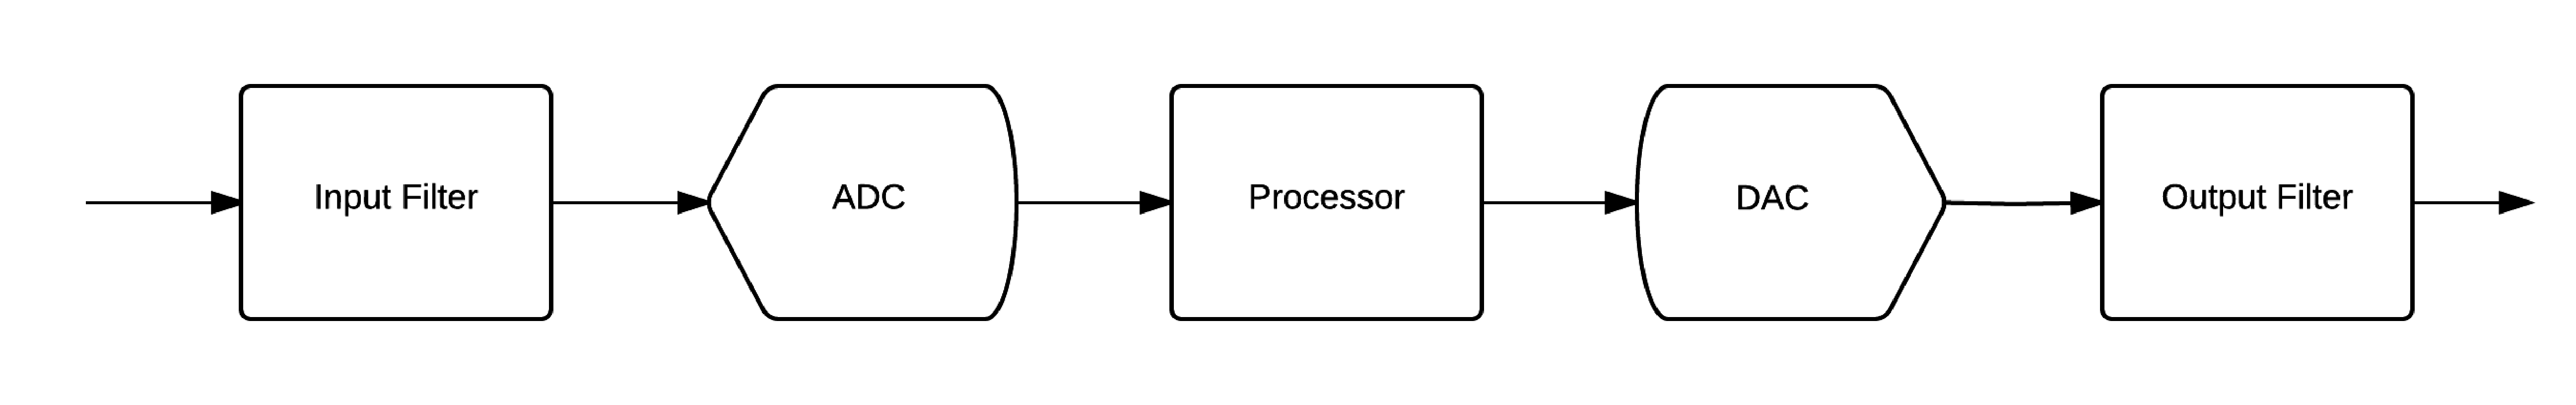
\includegraphics[width=0.8\textwidth]{./figures/sdr_basic_arch}
    \caption{ Software Defined Radio Basic Architecture
    \label{fig:sdr_basic}}
\end{figure}


Implementations may vary a lot, some common implementations are Made in matlab
through Simulink and use the computer’s video card as a medium of communication.
A more difficult but more interesting implementation involves the use of DSP
chips to implement the signal processing functions and some cheap ADC and DAC
chips can compose the SDR system.\\

The most commercial and famous implementation of SDR is Gnuradio+USRP, USRP
stands for Universal Software Radio Peripheral \cite{web:usrp} and Gnuradio
\cite{web:gnuradio} is a software for PC which has various digital signal
processing functions and modulation schemes and comes with a driver to use USRP.
The USRP itself is basically and FPGA hooked with a transceiver, so this pair is
broadly used in research and academic environments.\\

When we talk about research and development of real-world systems there is
always a tradeoff or bottleneck, in SDR the bottleneck is the hardware related
to the antenna interface, the antenna is designed to work better in a specific
bandwidth, this can limit the application, of course this is only one example of
bottleneck, there are others like Oscillator frequency, PLL, and processor
capability.\\

This work has a SDR like implementation done in FPGA and using the transceiver
AD9361 which makes baseband upconversion (Transmitter) and downconversion
(Receiver), filters and make analog to digital conversion and digital to analog
conversion, thus it is possible to implement transmitter and receiver with only
one board, however the most complex part does not lie in the system itself
because some electronic parts became a commodity, the complexity is in the
modulation/demodulation blocks and all the synchronization process, such topics
shall be discussed in the chapter \ref{cap:digitalcomm}.

\chapter{Long Term Evolution}
\label{chap:lte}

\section{Digital Communication System Overview}
\label{lte:digicomm}

The purpose of any Communication System is to transport an information bearing
signal from a source to a user destination via a communication channel. Being
Transmitter, Receiver and Channel the three basic elements of every
communication systems whose block diagram can be seen in figure \ref{fig:digicomsimple}.\\

%esquema básico do sistema de comunicação
\begin{figure}[htbp]
    \centering
    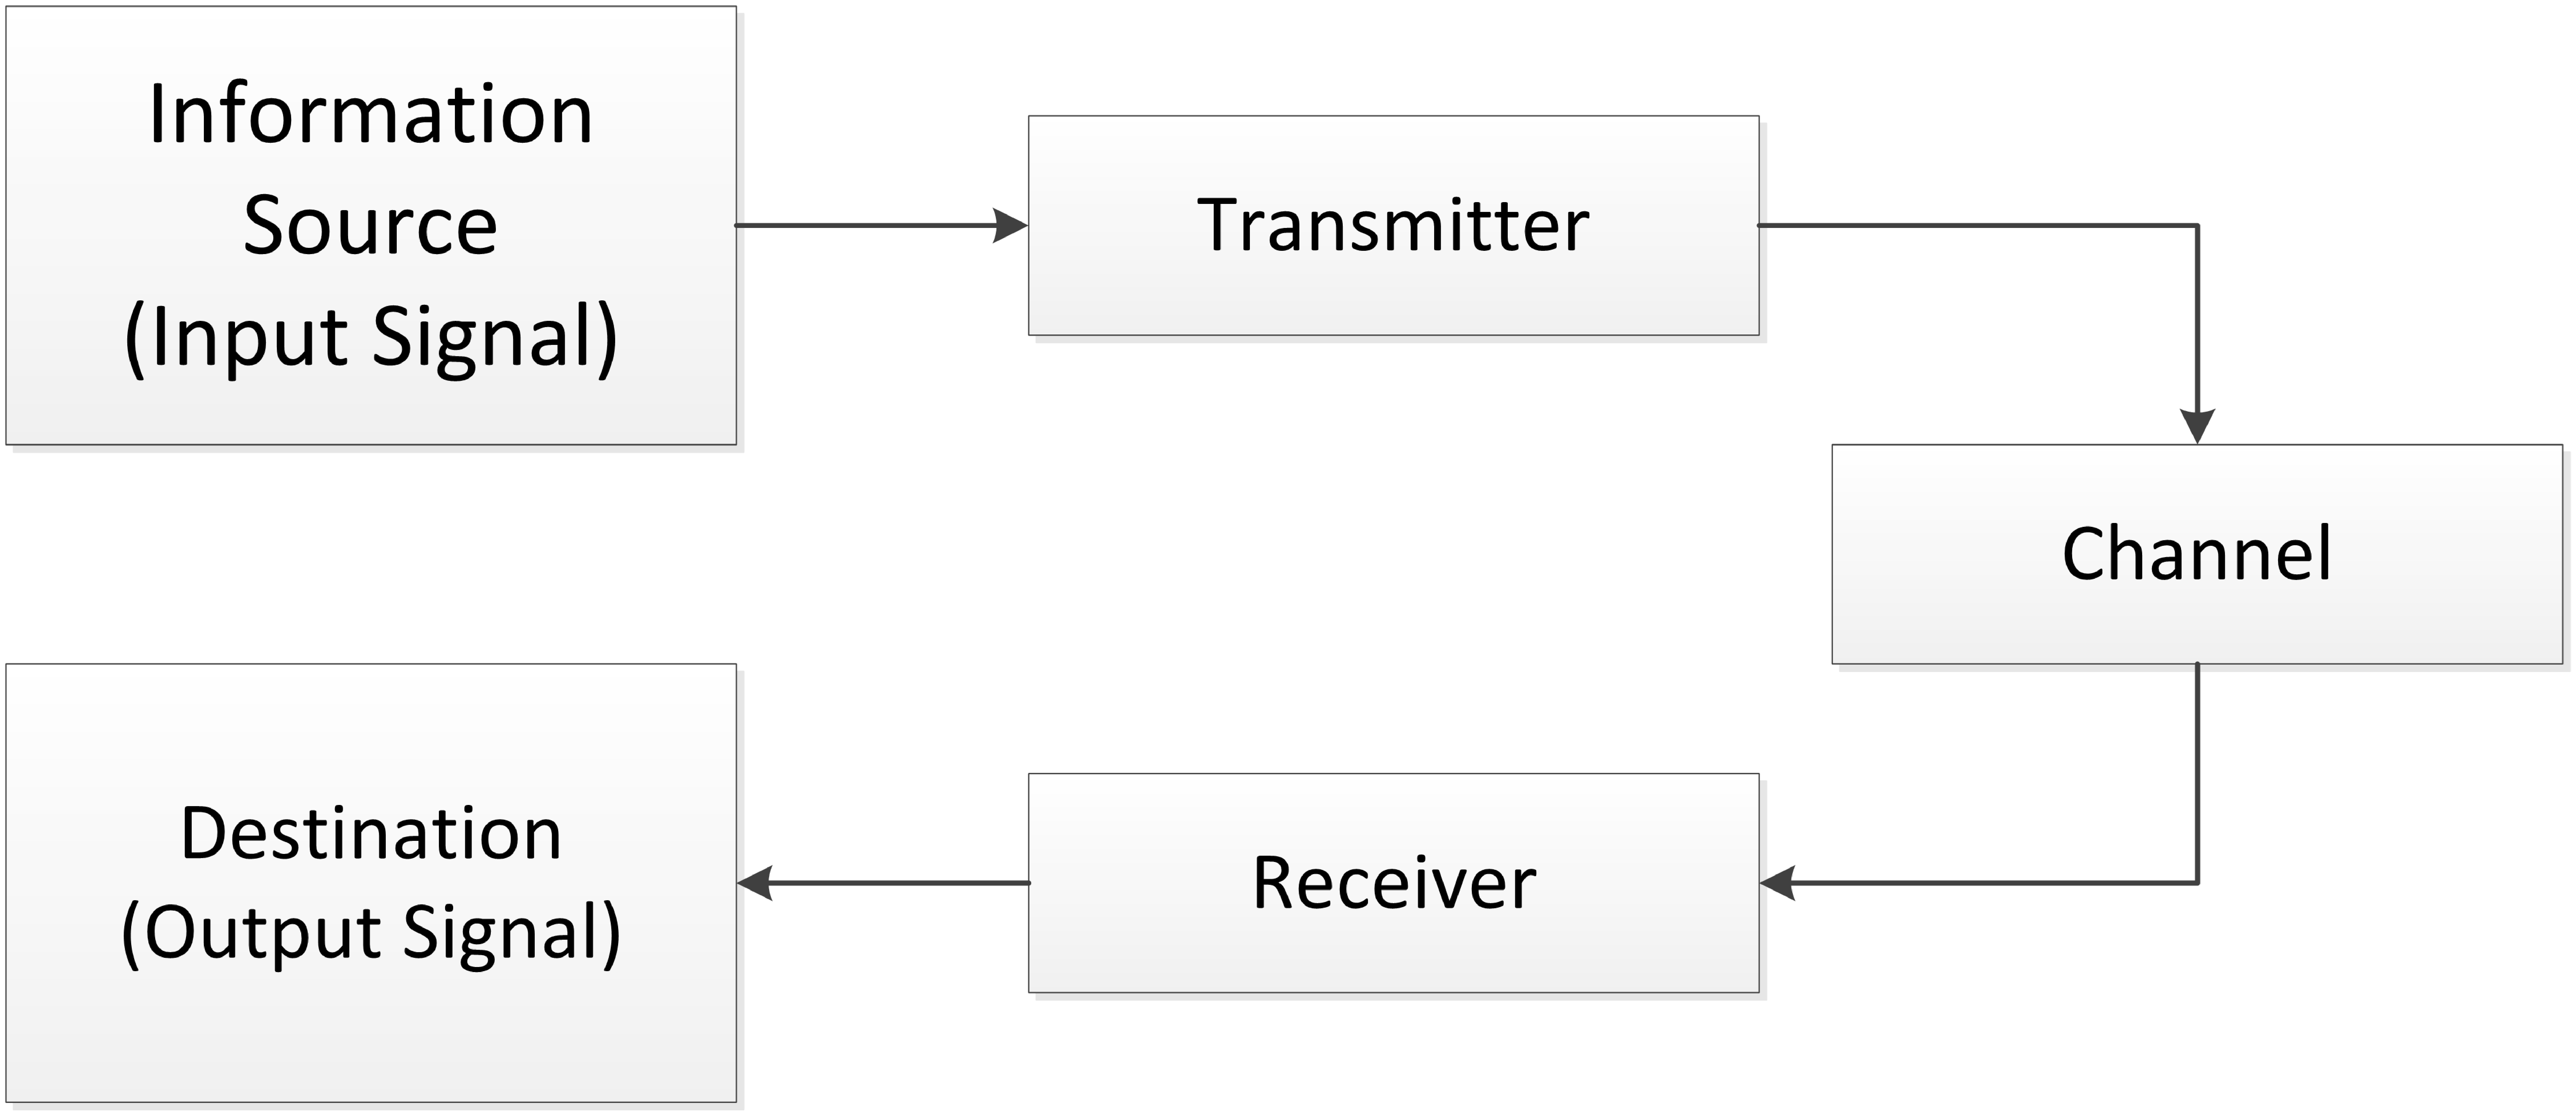
\includegraphics[width=0.65\textwidth]{./figures/digicom_simple}
    \caption{ A simple Digital Communication System Block Diagram
    \label{fig:digcomsimple}}
\end{figure}

The overall purpose of the system is to transfer information from one point (
Source) to another point, the destination.The message produced by a source,
normally, it is a digital message, usually binary, thus not electrical. Hence an
input transducer is used for converting the message to a time-varying electrical
quantity called message signal. Similarly, at the destination point,another
transducer converts the electrical waveform to the appropriate message.\\

The transmitter is located at one point in space, the receiver is located at
some other point separate from the transmitter, and the channel is the medium
that provides the electrical connection between them. Its purpose is to
transform the message signal produced by the source of information into a form
suitable for transmission over the channel.\\

The received signal is normally corrupted version of the transmitted signal,
which is due to channel imperfections, noise and interference from other
sources.It has the task of operating on the received signal so as to reconstruct
a recognizable form of the original message signal and to deliver it to the user
destination.\\

Communication Systems are divided into 3 categories:

\begin{enumerate}

  \item Analog Communication Systems are designed to transmit analog information
  using analog modulation methods, FM and AM, common radio.

  \item Digital Communication Systems are designed for transmitting digital
  information using digital modulation schemes, like FSK and PSK.

  \item Hybrid Systems that use digital modulation schemes for transmitting
  sampled and quantized values of an analog message signal.

\end{enumerate}

\subsection{Elements of Digital Communications Systems}

%block diagram of a digital communication system
\begin{figure}[htbp]
    \centering
    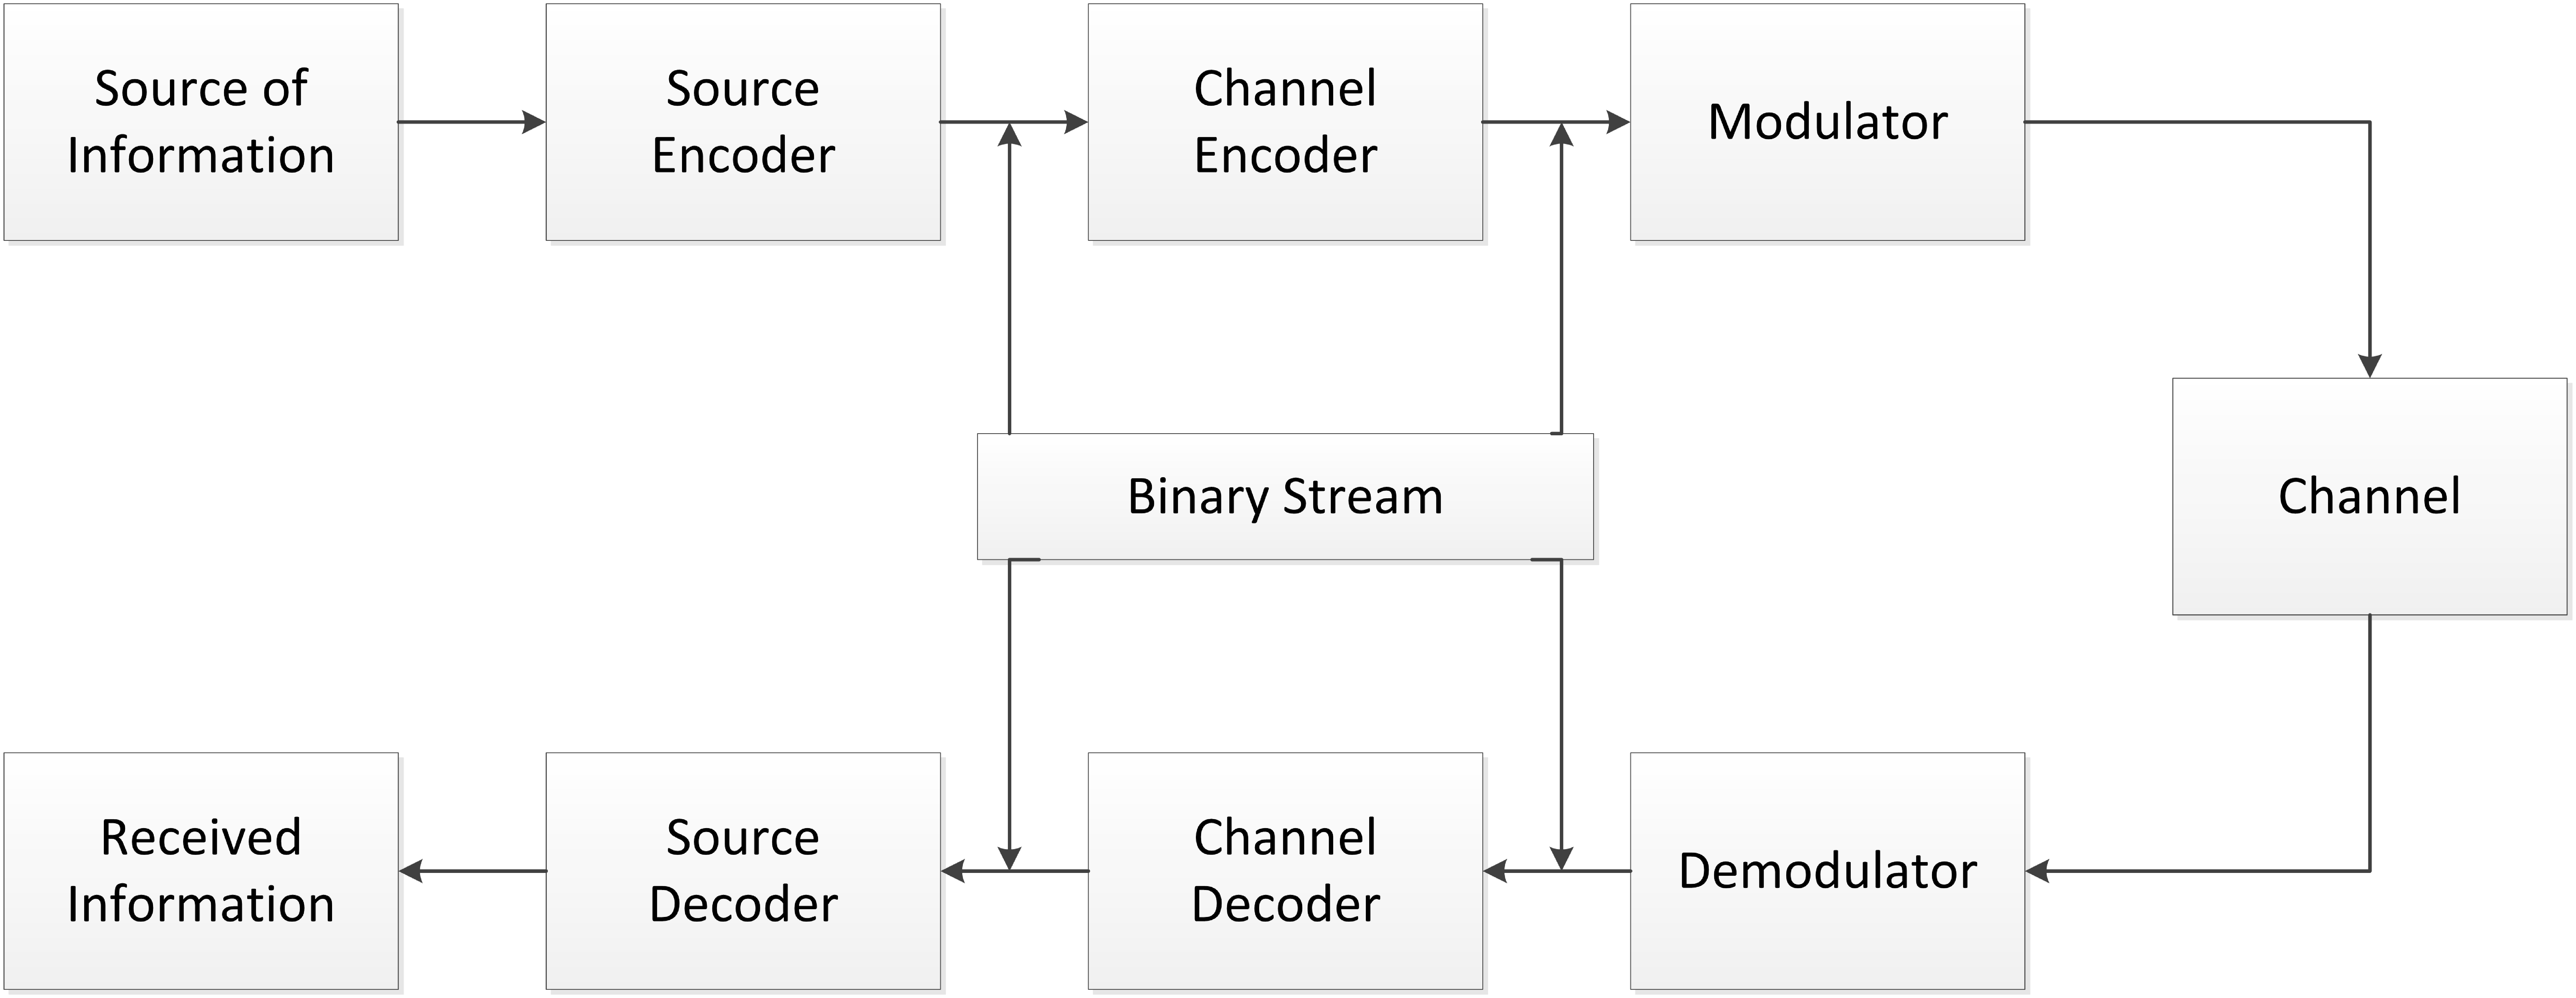
\includegraphics[width=0.85\textwidth]{./figures/digicom_bd}
    \caption{ Digital Communication System Block Diagram
    \label{fig:digcombd}}
\end{figure}

\subsubsection{Source of information}

The sources of information can be of two main kinds, \emph{Analog Information
sources} and \emph{Digital Information Sources}. The Analog information sources
are, for example, microphones and cathodic ray tube televisions, usually any
device that have to reproduce or record anything in the real-world is analogic,
because the real world is analogic. \\

In the other side there are the digital information sources which are composed
by a discrete sequence of symbols, thus the main digital information source is
the PC.

\subsubsection{Source Encoder / Decoder}

The \emph{Source encoder}  and \emph{Source coder} converts the input symbol
sequence into a binary sequence (0 and 1) by assigning code words to the symbols
in the input sequence.\\

If a source set is having hundred symbols, then the number of bits used to
represent each symbol will be 7 because $27=128$ unique combinations are
available. The important parameters of a source encoder are block size, code
word lengths, average data rate and the efficiency of the coder, which is the
actual output data rate compared to the minimum achievable rate.\\

At the receiver, the source decoder converts the binary output of the channel
decoder into a symbol sequence. The decoder for a system using fixed length code
words is quite simple, but the decoder for a system using variable length code
words will be very complex.\\

Aim of the source coding is to remove the redundancy in the transmitting
information, so that bandwidth required for transmission is minimized. Based on
the probability of the symbol codeword is assigned. Higher the probability,
shorter is the codeword.

\subsubsection{Channel Encoder / Decoder}

Error control is accomplished by the channel coding operation that consists of
systematically adding extra bits to the output of the source coder. These extra
bits do not convey any information but helps the receiver to detect and / or
correct some of the errors in the information bearing bits.\\

There are two methods of channel coding:

\begin{enumerate}

  \item \textbf{Block Coding:} The encoder takes a block of ‘k’ information bits
  from the source encoder and adds ‘r’ error control bits, where ‘r’ is dependent
  on ‘k’ and error control capabilities desired.

  \item \textbf{Convolution Coding:} The information bearing message stream is
  encoded in a continuous fashion by continuously interleaving information bits
  and error control bits.

\end{enumerate}


The Channel decoder recovers the information bearing bits from the coded binary
stream. Error detection and possible correction is also performed by the channel
decoder.

\subsubsection{Modulator}

The Modulator converts the input bit stream into an electrical waveform suitable
for transmission over the communication channel, the carrier wave. Modulator can
be effectively used to minimize the effects of channel noise, to match the
frequency spectrum of transmitted signal with channel characteristics, to
provide the capability to multiplex many signals.

\subsubsection{Demodulator}

The extraction of the message from the information bearing waveform produced by
the modulation is accomplished by the demodulator. The output of the demodulator
is bit stream.

\subsubsection{Channel}

The Channel provides the electrical connection between the source and
destination. The different channels are: Pair of wires, Coaxial cable, Optical
fibre, Radio channel, Satellite channel or combination of any of these.\\

The communication channels have only finite Bandwidth, non-ideal frequency
response, the signal often suffers amplitude and phase distortion as it travels
over the channel. Also, the signal power decreases due to the attenuation of the
channel. The signal is corrupted by unwanted, unpredictable electrical signals
referred to as noise. The important parameters of the channel are Signal to
Noise power Ratio (SNR), usable bandwidth, amplitude and phase response and the
statistical properties of noise.

\subsection{Additional Blocks}
%augmented block diagram
\begin{figure}[htbp]
    \centering
    
\includegraphics[width=0.85\textwidth]{./figures/digicom_plus}
    \caption{ Digital Communication System Block Diagram with additional blocks
    \label{fig:digcomplus}}
\end{figure}

Some additional blocks as shown in the block diagram  at figure \ref{fig:digicomplus}
are used in most of digital communication system:

\begin{itemize}

  \item \textbf{Encryptor:} Encryptor prevents unauthorized users from
understanding the messages and from injecting false messages into the system.

  \item \textbf{Multiplexer:} Multiplexer is used for combining signals from
different sources so that they share a portion of the communication system.

  \item \textbf{Demultiplexer:} DeMultiplexer is used for separating the different
signals so that they reach their respective destinations.

  \item \textbf{Decryptor:} It does the reverse operation of that of the Encryptor.

\end{itemize}

\subsection{Synchronization}

Synchronization involves the estimation of both time and frequency coherent
systems need to synchronize their frequency reference with carrier in both
frequency and phase.

\subsection{Advantages and Disadvantages}

Advantages:

\begin{enumerate}

  \item The effect of distortion, noise and interference is less in a digital
  communication system. This is because the disturbance must be large enough to
  change the pulse from one state to the other.

  \item Regenerative repeaters can be used at fixed distance along the link, to
  identify and regenerate a pulse before it is degraded to an ambiguous state.

  \item Digital circuits are more reliable and cheaper compared to analog
  circuits.

  \item The Hardware implementation is more flexible than analog hardware because
  of the use of microprocessors, VLSI chips etc.

  \item Signal processing functions like encryption, compression can be employed
  to maintain the secrecy of the information.

  \item Error detecting and Error correcting codes improve the system performance
  by reducing the probability of error.

  \item Combining digital signals using TDM is simpler than combining analog
  signals using FDM. The different types of signals such as data, telephone, TV
  can be treated as identical signals in transmission and switching in a digital
  communication system.

  \item We can avoid signal jamming using spread spectrum technique.

\end{enumerate}

Disadvantages:

\begin{enumerate}

  \item \textbf{Large System Bandwidth:} Digital transmission requires a large system
  bandwidth to communicate the same information in a digital format as compared to
  analog format.

  \item \textbf{System Synchronization:} Digital detection requires system synchronization
  whereas the analog signals generally have no such requirement.

\end{enumerate}

%-----------------------------------LTE-----------------------------------------

\section{Long Term Evolution} %OK
\label{let:lte}

\subsection{Overview}

Long Term Evolution (LTE) is a standard for wireless communication for high-speed
mobile devices and data terminals. LTE was first introduced in 3GPP Release 8.
It uses orthogonal frequency division multiplexing (OFDM) as its radio access
technology, together with advanced antenna technologies.\\

In addition to LTE, 3GPP also defined IP-based, flat core network architecture.
This architecture was defined as part of the System Architecture Evolution (SAE)
effort specifying the Evolved Packet Core (EPC) network. The LTE-SAE architecture
and concepts have been designed for efficient support of mass-market usage of any
IP-based service. The architecture is based on an evolution of the existing GSM/WCDMA
core network, with simplified operations and smooth, cost-efficient deployment.\\

Moreover, work has also been done by 3GPP in cooperation with 3GPP2 (the CDMA
standardization body) to optimize interworking between CDMA and LTE-SAE. This means
that both CDMA and GSM operators can use the same standard with minor modifications
and thus making the deployment and roaming costs smaller.\\

LTE can be was thought to reduce cost in deployment in legacy systems, as said
before with CDMA and GSM, it can use the legacy systems and adapt itself to work
with them, creating a smooth transition for the network operators \cite{introlte}.\\

The 3GPP radio access  technology was developed towards:

\begin{itemize}
    \item Reduced cost per bit
    \item Increased service provisioning – more services at a lower cost with
    better user experience
    \item Flexible use of existing and new frequency bands
    \item Simplified architecture and open interfaces
    \item Reasonable terminal power consumption
\end{itemize}

The specification work on LTE was completed in March 2009 as the SAE specifications
were included. Below it is possible to see some of the 3GPP Release 8 LTE Requirements:

\begin{itemize}
    \item Increased peak data rates: 100Mbps downlink and 50Mbps uplink
    \item Reduction of Radio Access Network (RAN) latency to 10ms
    \item Improved spectrum efficiency (two to four times compared with HSPA Release 6)
    \item Cost-effective migration from Release 6 Universal Terrestrial Radio
    Access (UTRA) radio interface and architecture
    \item Improved broadcasting
    \item IP-optimized (focus on services in the packet switched domain)
    \item Scalable bandwidth of 20MHz, 15MHz, 10MHz, 5MHz, 3MHz and 1.4MHz
    \item Support for both paired and unpaired spectrum
    \item Support for interworking with existing 3G systems and non-3GPP specified systems.
\end{itemize}

\subsection{Network Architecture}

In parallel with the LTE radio access, the packet core network was implemented as
flat IP-based multi-access core network. The Evolved Packet Core (EPC) network was
designed to optimize network performance, improve cost-efficiency and facilitate
the uptake of mass-market multimedia services.\\

Existing 3GPP (GSM and WCDMA/HSPA) and 3GPP2 (CDMA2000 1xRTT, EV-DO) systems are
integrated to the EPC network through standardized interfaces providing optimized
mobility with LTE. For 3GPP systems this means a signaling interface between the
existing Serving GPRS Support Node (SGSN) to the Mobility Management Entity (MME)
in the EPC network; for 3GPP2 a control signaling interface between the CDMA RAN
and the MME. This integration support both dual and single radio handover, allowing
a flexible migration to LTE.\\

The Home Subscriber Server (HSS) connects to the Packet Core through an IP-based
interface using Diameter, and not SS7, which was used in previous GSM and WCDMA
networks. Network signaling for policy control and charging is already based on
Diameter. This means that all interfaces in the new architecture are IP-based.\\

LTE-EPC has adopted an effective class-based QoS concept. This provides a
foundation for operators to offer service differentiation, depending on the type
of subscription or application.

%figura da rede
\begin{figure}[htbp]
    \centering
    
\includegraphics[width=0.65\textwidth]{./figures/lte_flatepc}
    \caption{ LTE Flat EPC Network Architecture
    \label{fig:lteflatepc}}
\end{figure}

\subsection{Orthogonal Frequency-division Multiplexing Radio Technology} %+/-ok

LTE uses OFDM for the downlink ( from the base station to the terminal or UE).
OFDM meets the LTE requirement for spectrum flexibility and enables cost-efficient
solutions for very wide carriers with high peak rates. It is a well-established
technology: for example, in standards such as IEEE 802.11a/b/g, 802.16, HIPERLAN-2,
DVB and DAB.\cite{introlte} \cite{umtslte}\\

A representation of an OFDM signal can be seen in figure \ref{fig:ofdmfreq}. In
this figure, a signal with 5 MHz bandwidth is shown, but the principle is of
course the same for the other E-UTRA bandwidths. Data symbols are independently
modulated and transmitted over a high number of closely spaced orthogonal
subcarriers.\\

%ofdm scheme
\begin{figure}[htbp]
    \centering
    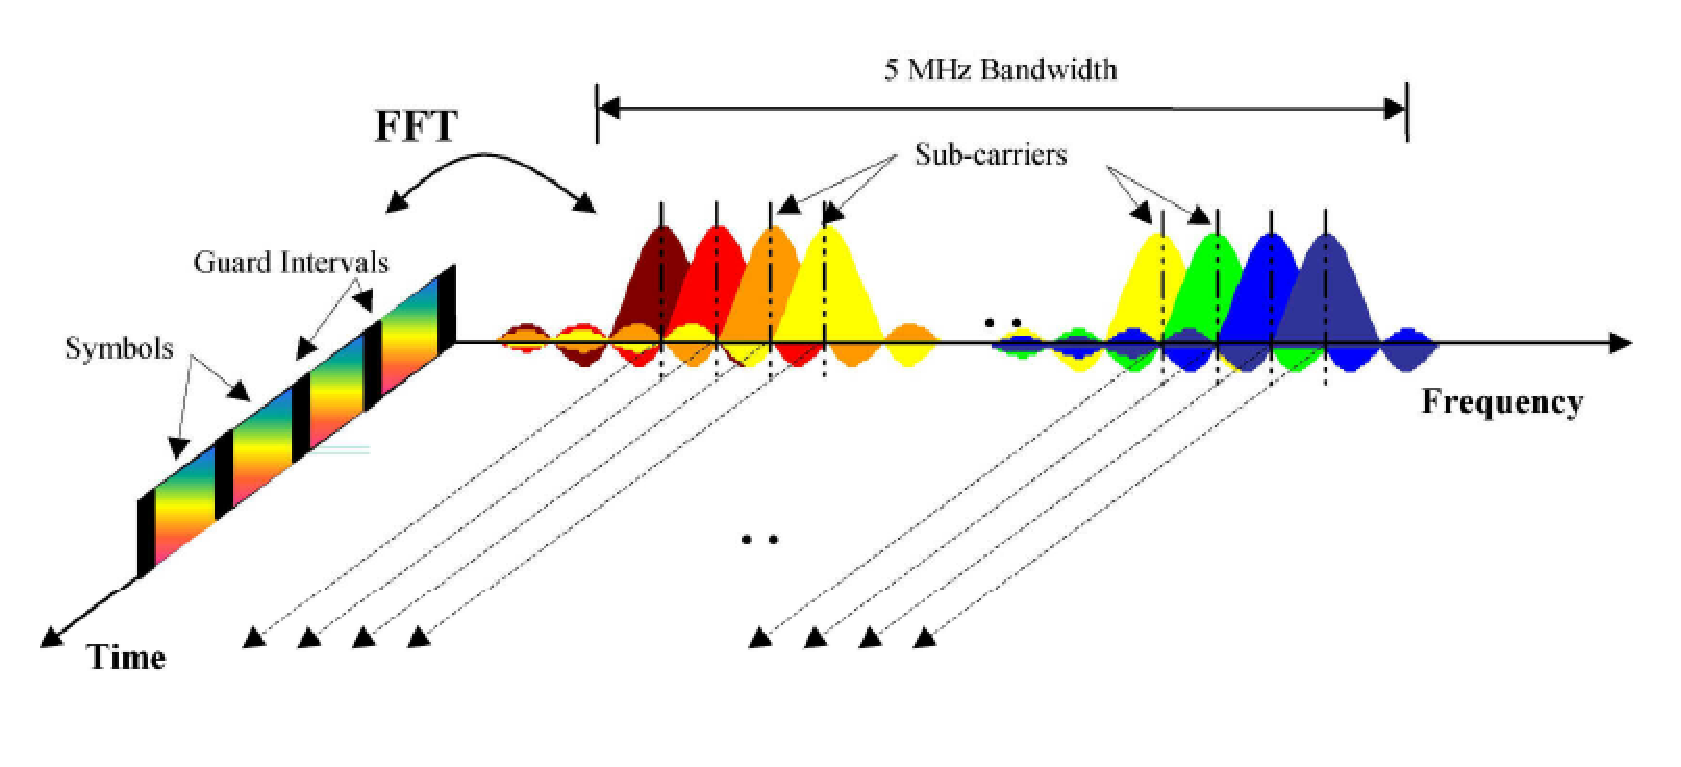
\includegraphics[width=0.65\textwidth]{./figures/ofdm_frequency}
    \caption{ Frequency-Time Representation of OFDM signal
    \label{fig:ofdmfreq}}
\end{figure}

OFDM uses a large number of narrow sub-carriers for multi-carrier transmission.
The basic LTE downlink physical resource can be seen as a time-frequency grid.
In the frequency domain, the spacing between the sub-carriers, $\Delta f$, is 15
kHz. In addition, the OFDM symbol duration time is $\frac{1}{\Delta f} + cyclic prefix$.
The cyclic prefix is used to maintain orthogonality between the sub-carriers even
for a time-dispersive radio channel. One resource element carries QPSK, 16QAM or
64QAM. With 64QAM, each resource element carries six bits.\\

The OFDM symbols are grouped into resource blocks. The resource blocks have a
total size of 180 kHz in the frequency domain and 0.5ms in the time domain. Each
user is allocated a number of so-called resource blocks in the time-frequency grid.
The more resource blocks a user gets, and the higher the modulation used in the
resource elements, the higher the bit rate. Which resource blocks the user gets
at a given point in time, and how many, depends on advanced scheduling mechanisms
in the frequency and time dimensions.\\

Scheduling of resources can be taken every 1ms: that means two resource blocks,
180 kHz wide and in total 1ms in length (called a Scheduling Block). The scheduling
mechanisms in LTE are similar to those used in HSPA, and enable optimal performance
for different services in different radio environments.\\

In the uplink, LTE uses a pre-coded version of OFDM called Single Carrier Frequency
Division Multiple Access (SC-FDMA). This is to compensate for a drawback with normal
OFDM, which has a very high Peak to Average Power Ratio (PAPR). High PAPR requires
expensive and inefficient power amplifiers with high linearity requirements, which
increases the cost of the terminal and drains the battery faster.\\

SC-FDMA solves this problem by grouping together the resource blocks in such a
way that it reduces the need for linearity, and so power consumption, in the
power amplifier. A low PAPR also improves coverage and cell-edge performance.

Since this work shall focus on the Radio Frontend part of the systems, implementing
a downlink scheme, it is interesting to dwell more in the LTE downlink and uplink
schemes.

\subsection{Downlink Scheme}%OK

The downlink transmission scheme for E-UTRA FDD and TDD modes is based on
conventional OFDM. In an OFDM system, the available spectrum is divided into
multiple carriers, called subcarriers as explained in the previus section. Each
of these subcarriers is independently modulated by a low rate data stream. OFDM
is used as well in WLAN, WiMAX and broadcast technologies like DVB (Digital
Video Broadcasting). OFDM has several benefits including its robustness against
multipath fading and its efficient The user data is carried on the Physical Downlink Shared Channel (PDSCH). The
PDSCH(s) is the only channel that can be QPSK, 16QAM or 64QAM modulated. The
Downlink channel schematic can be seen in \ref{fig:dlchann}to channels delay spread. The delay spread is
the time between the symbol arriving on the first multi-path signal and the last
multi-path signal component, typically several $\mu s$ dependent on the environment
(i.e. indoor, rural, suburban, city center). The guard interval has to be selected
in that way, that it is greater than the maximum expected delay spread. In E-UTRA,
the guard interval is a cyclic prefix which is inserted prior to each OFDM symbol.\\

In practice, the OFDM signal can be generated using IFFT (Inverse Fast Fourier Transform)
digital signal processing. The IFFT converts a number N of complex data
symbols used as frequency domain bins into the time domain signal. Such an N-point
IFFT is illustrated in Figure X where $a(mN+n)$ refers to the nth subcarrier
modulated data symbol, during the time period $mTu < t £ (m+1)Tu$.

%ofdm symbols
\begin{figure}[htbp]
    \centering
    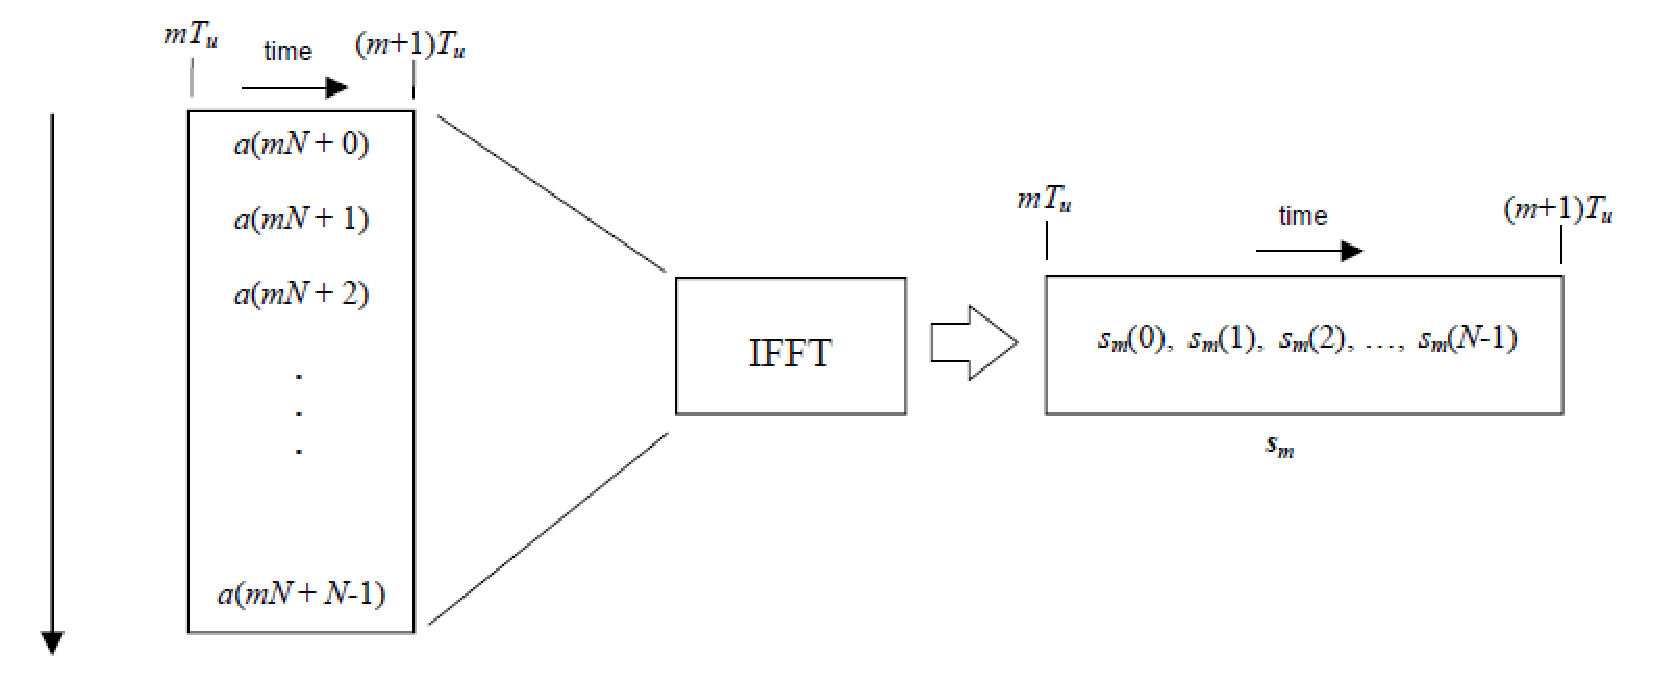
\includegraphics[width=0.65\textwidth]{./figures/ofdm_symbol_gen}
    \caption{ OFDM Symbol Generation
    \label{fig:ofdmsymbol}}
\end{figure}

The vector $sm$ is defined as the useful OFDM symbol. It is the time superposition
of the $N$ narrowband modulated subcarriers. Therefore, from a parallel stream
of $N$ sources of data, each one independently modulated, a waveform composed of
N orthogonal subcarriers is obtained, with each subcarrier having the shape of a
frequency sinc function. Figure 4 illustrates the mapping from a
serial stream of QAM symbols to N parallel streams, used as frequency domain bins
for the IFFT. The N-point time domain blocks obtained from the IFFT are then
serialized to create a time domain signal.

%ofdm signal chain
\begin{figure}[htbp]
    \centering
    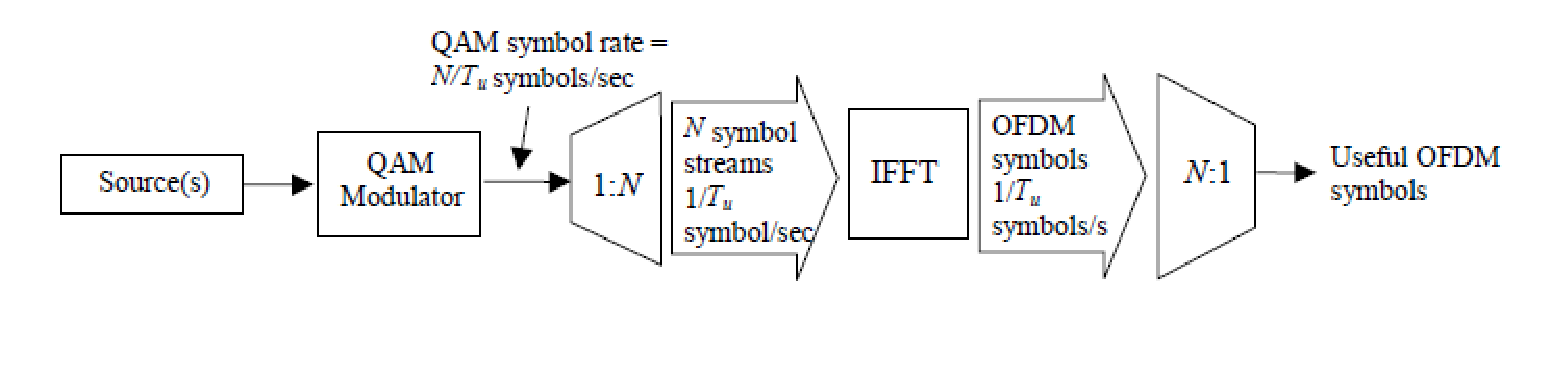
\includegraphics[width=0.65\textwidth]{./figures/ofdm_signal_chain}
    \caption{ OFDM Signal Generation
    \label{fig:ofdmchain}}
\end{figure}

In contrast to an OFDM transmission scheme, OFDMA allows the access of multiple
users on the available bandwidth. Each user is assigned a specific time-frequency
resource.

As stated before the data is allocated to a device (User Equipment, UE) in terms
of resource blocks, this means that one UE can be allocated integer multiples of
one resource block in the frequency domain, which representation can be seen in
figure \ref{fig:ofdmresblk}. These resource blocks do not have to be adjacent to
each other. In the time domain, the scheduling decision can be modified every
transmission time interval of 1 ms. All scheduling decisions for downlink and
uplink are done in the base station (enhanced NodeB, eNodeB or eNB). The
scheduling algorithm has to take into account the radio link quality situation
of different users, the overall interference situation, Quality of Service
requirements, service priorities, etc. and is a vendor-specific implementation.
Figure 8 shows an example for allocating downlink user data to different
users.\\

%ofdm resource block
\begin{figure}[htbp]
    \centering
    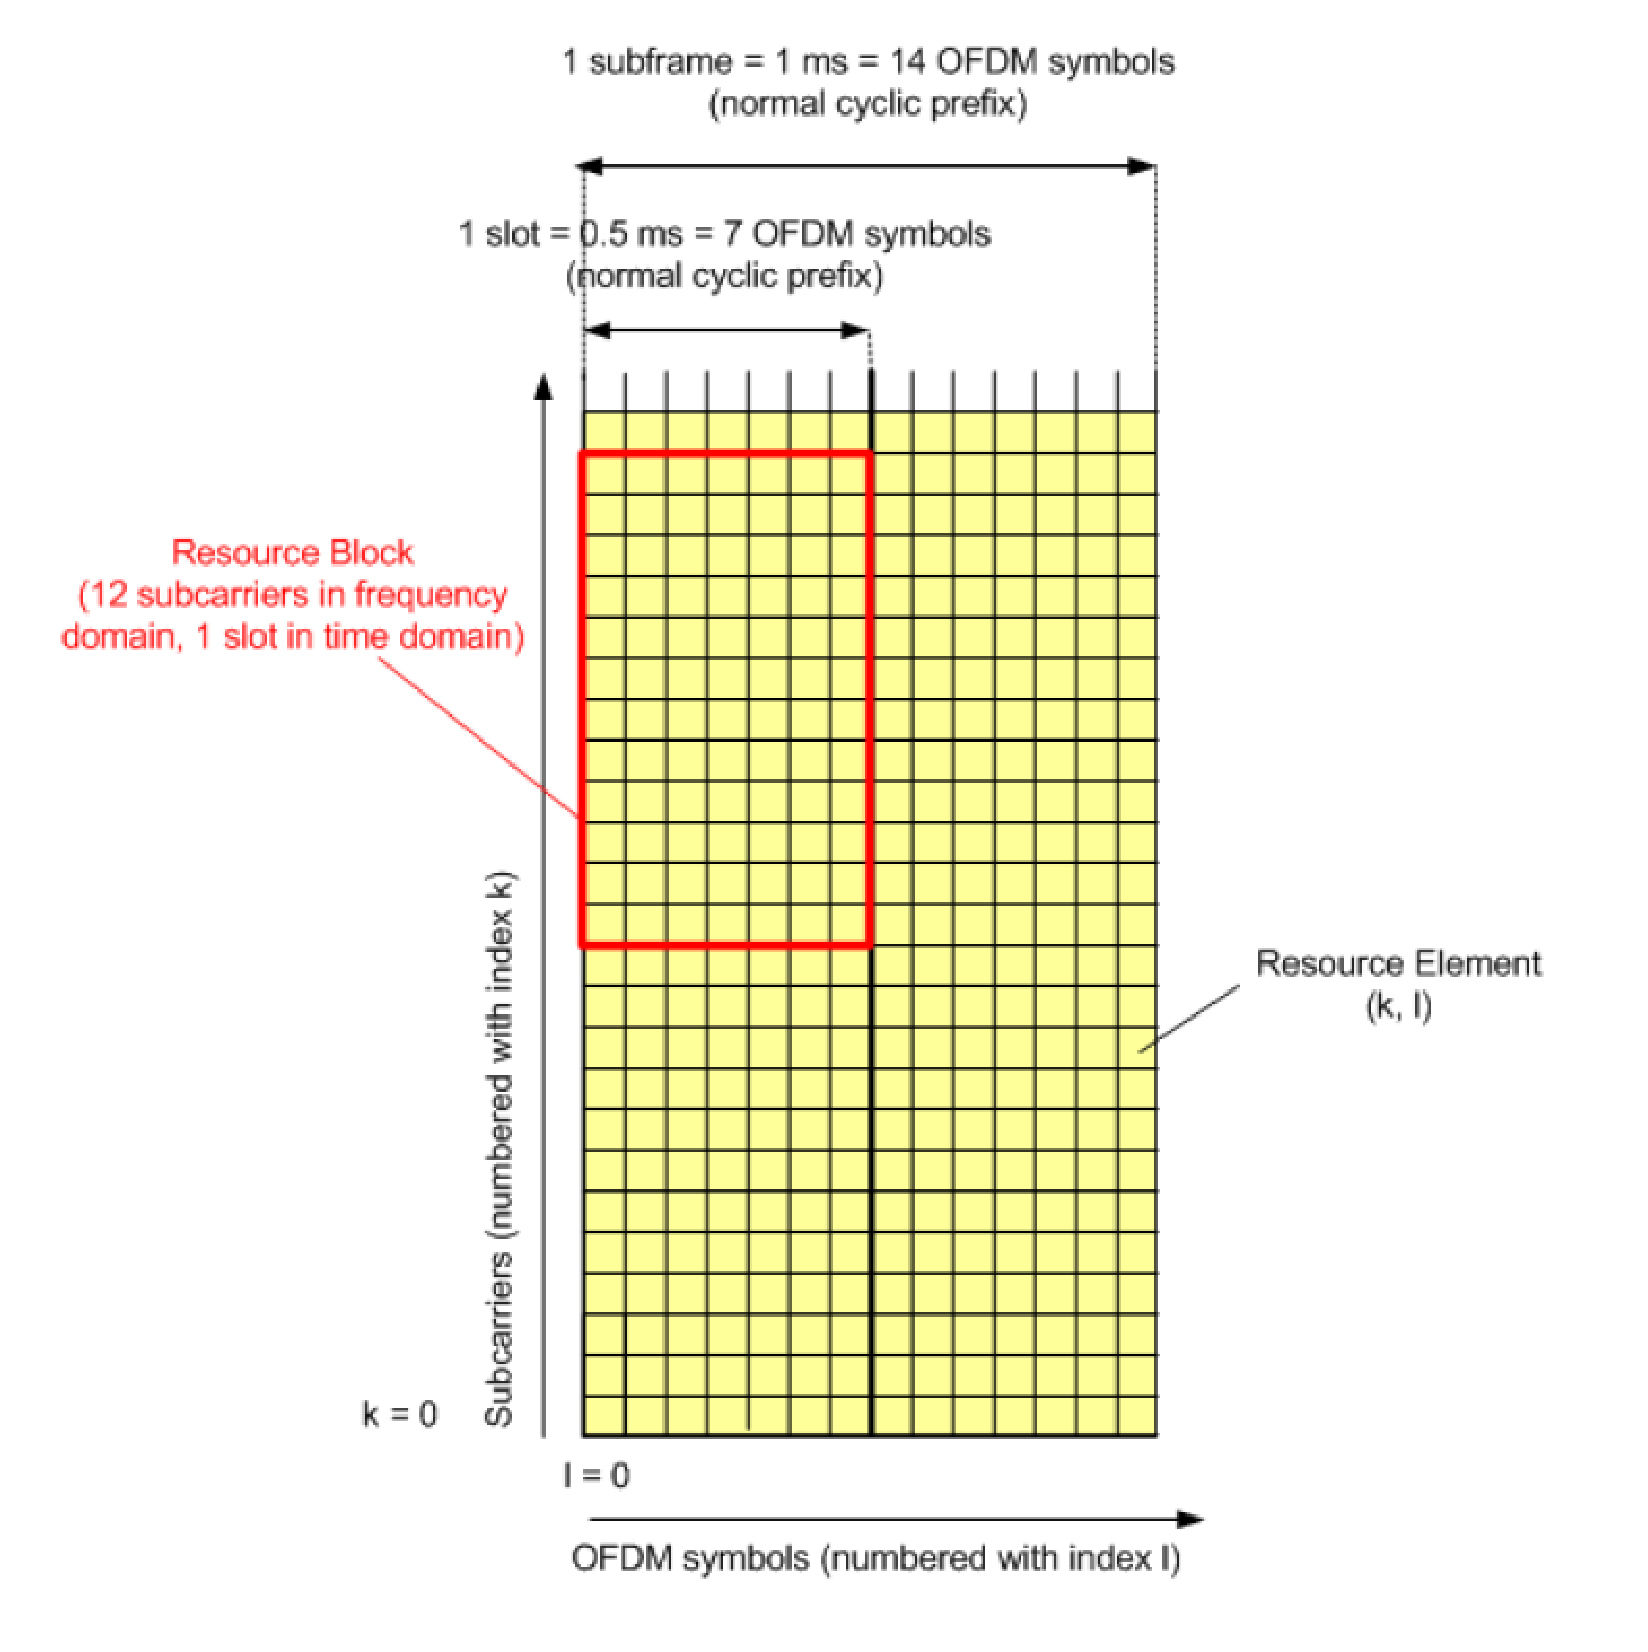
\includegraphics[width=0.65\textwidth]{./figures/ofdm_resource_block}
    \caption{ Resource Block Organization Example
    \label{fig:ofdmresblk}}
\end{figure}

The user data is carried on the Physical Downlink Shared Channel (PDSCH). The
PDSCH(s) is the only channel that can be QPSK, 16QAM or 64QAM modulated. The
Downlink channel schematic can be seen in \ref{fig:dlchann}

%downlink channel figura
\begin{figure}[htbp]
    \centering
    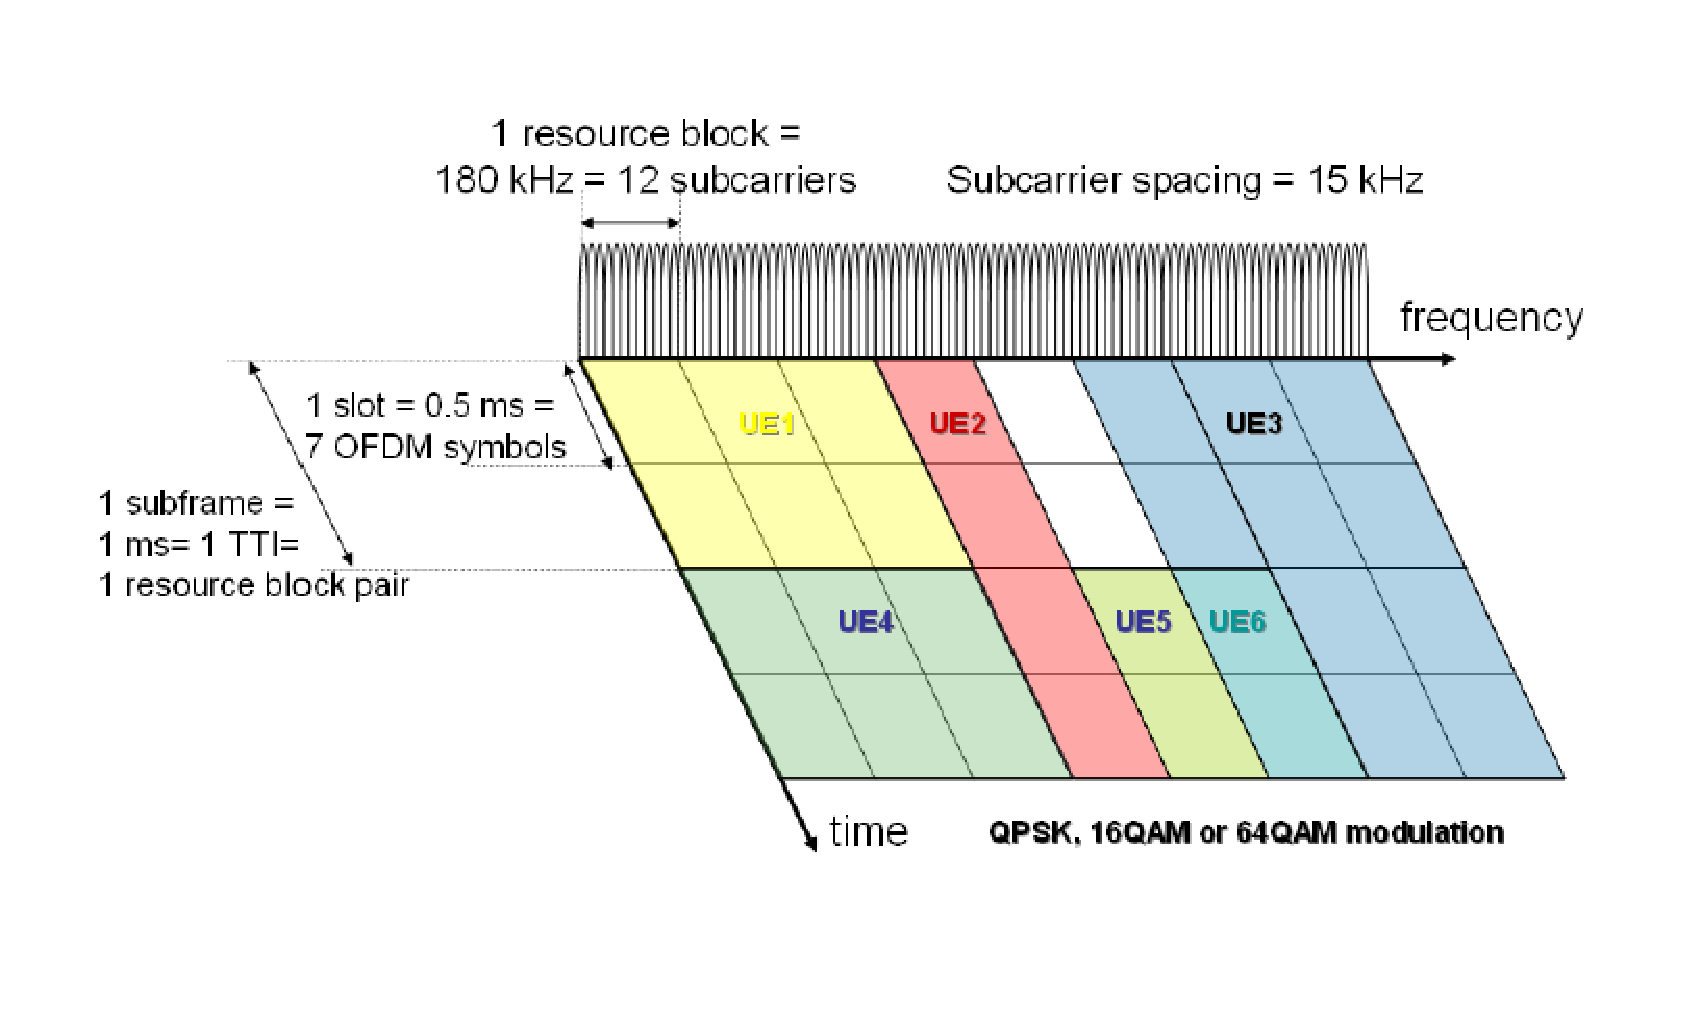
\includegraphics[width=0.65\textwidth]{./figures/downlink_channels}
    \caption{ OFDMA time-frequency multiplexing
    \label{fig:dlchann}}
\end{figure}

\subsection{Uplink Scheme}%ok?

During the study item phase of LTE, alternatives for the optimum uplink transmission
scheme were investigated. While OFDMA is seen optimum to fulfill the LTE
requirements in downlink, OFDMA properties are less favorable for the uplink. This is
mainly due to weaker peak-to-average power ratio (PAPR) properties of an OFDMA
signal, resulting in worse uplink coverage and challenges in power amplifier design for
battery operated handset, as it requires very linear power amplifiers.\\

Thus, the LTE uplink transmission scheme for FDD and TDD mode is based on SC-
FDMA (Single Carrier Frequency Division Multiple Access) with cyclic prefix. SCFDMA
signals have better PAPR properties compared to an OFDMA signal. This was
one of the main reasons for selecting SC-FDMA as LTE uplink access scheme. The
PAPR characteristics are important for cost-effective design of UE power amplifiers.
Still, SC-FDMA signal processing has some similarities with OFDMA signal processing,
so parameterization of downlink and uplink can be harmonized.\\

There are different possibilities how to generate an SC-FDMA signal. DFT-spread-
OFDM (DFT-s-OFDM) has been selected for E-UTRA. For
DFT-s-OFDM, a size-M DFT is first applied to a block of M modulation
symbols. QPSK, 16QAM and 64QAM are used as uplink E-UTRA modulation
schemes, the latter being optional for the UE. The DFT transforms the modulation
symbols into the frequency domain. The result is mapped onto the available number
of subcarriers. For LTE Release 8 uplink, only localized transmission on consecutive
subcarriers is allowed. An N-point IFFT where N>M is then performed as in OFDM,
followed by addition of the cyclic prefix and parallel to serial conversion.

%figura uplink
\begin{figure}[htbp]
    \centering
    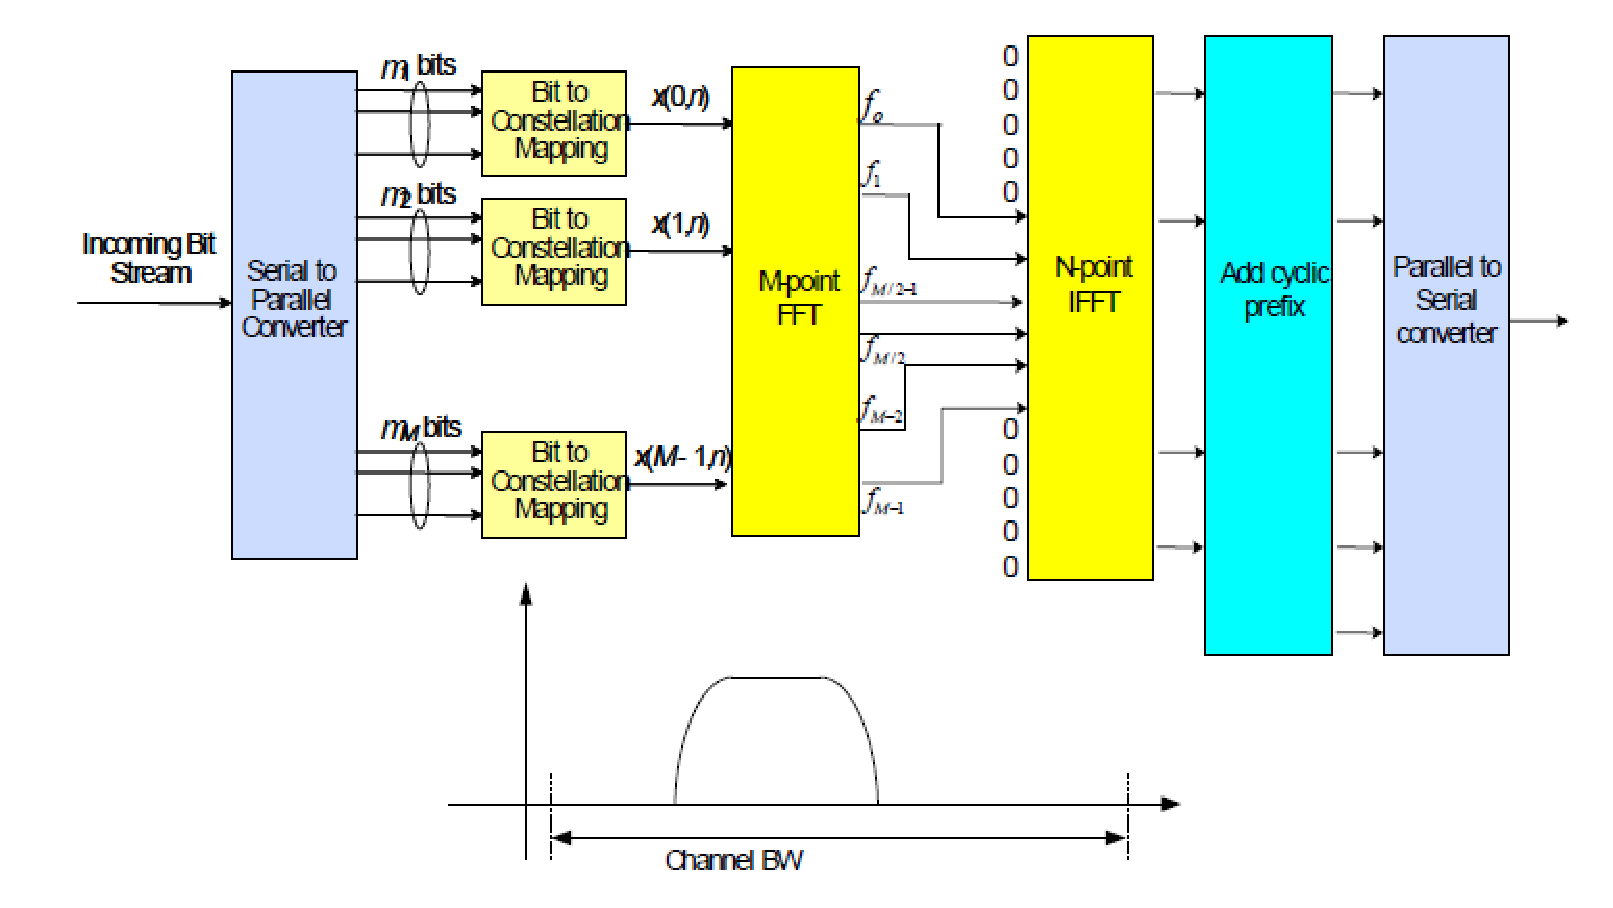
\includegraphics[width=0.65\textwidth]{./figures/uplink_scheme}
    \caption{ LTE Uplink Block diagram of DFT-s-OFDM
    \label{fig:uplinkbd}}
\end{figure}


\part{Implementation}
\chapter{FMComms2}
\section{AD9361}
\label{sec:ad9361}

The AD9361 is a high performance RF transceiver. Its programmability and adaptability makes it ideal for a wide range of transceiver applications. This device combines a RF front end with a flexible and configurable mixed-signal baseband section and frequency synthesizers, simplified configuration digital interface to a processor. 
The AD9361 operates from 70 MHz to 6.0GHz range with supported channel bandwidths from 200 KHz to 56 MHz and the AD9361 is a 2 Rx and 2 Tx device packed in a 10mm x10mm, 144 ball chip package ball grid array (CSP\_BGA).

\subsection{General Description}

AD9361 is a highly integrated RF frequency transceiver capable of being configured for a wide range of applications, including 3g and 4g frequency applications. AD9361 and AD9364 almost the same hardware and specifications, the difference is that AD9361 is a 2x2 MIMO and AD9364 is a 1x1 \cite{ad9361_wiki}.
The programmability allows the AD9361 to be operated in Frequency Division Duplex (FDD) and Time Division Duplex (TDD) systems, allowing this transceiver to operate in a variety of communication standards. Another interesting feature is the capability of integration with a wide range of BBPs (Baseband Processors) using a single or dual 12-bit parallel data port or a 12-bit LVDS (Low voltage Differential signaling), which uses the FMC connector in the FMCommS2 \ref{sec:fmcomms2}.
AD9361 also provides self-calibration and automatic gain control (AGC) systems to maintain good performance under variable conditions, such as temperature and signal quality. The transceiver has also various modes of test mode with the Built-in Self Test (BIST) modes which can be used for the designers to debug desgs during prototyping.
This configurability and adaptability is very attractive for Software Defined Radio (SDR) and for C-RAN systems, indeed ad9361 is already being used in some Universal Software Radio Peripheral (USRP) from ettus research (National Instruments), this alone is a proof that AD9361 can work in a wide range of systems and standards.

\begin{figure}[htbp]
    \centering
    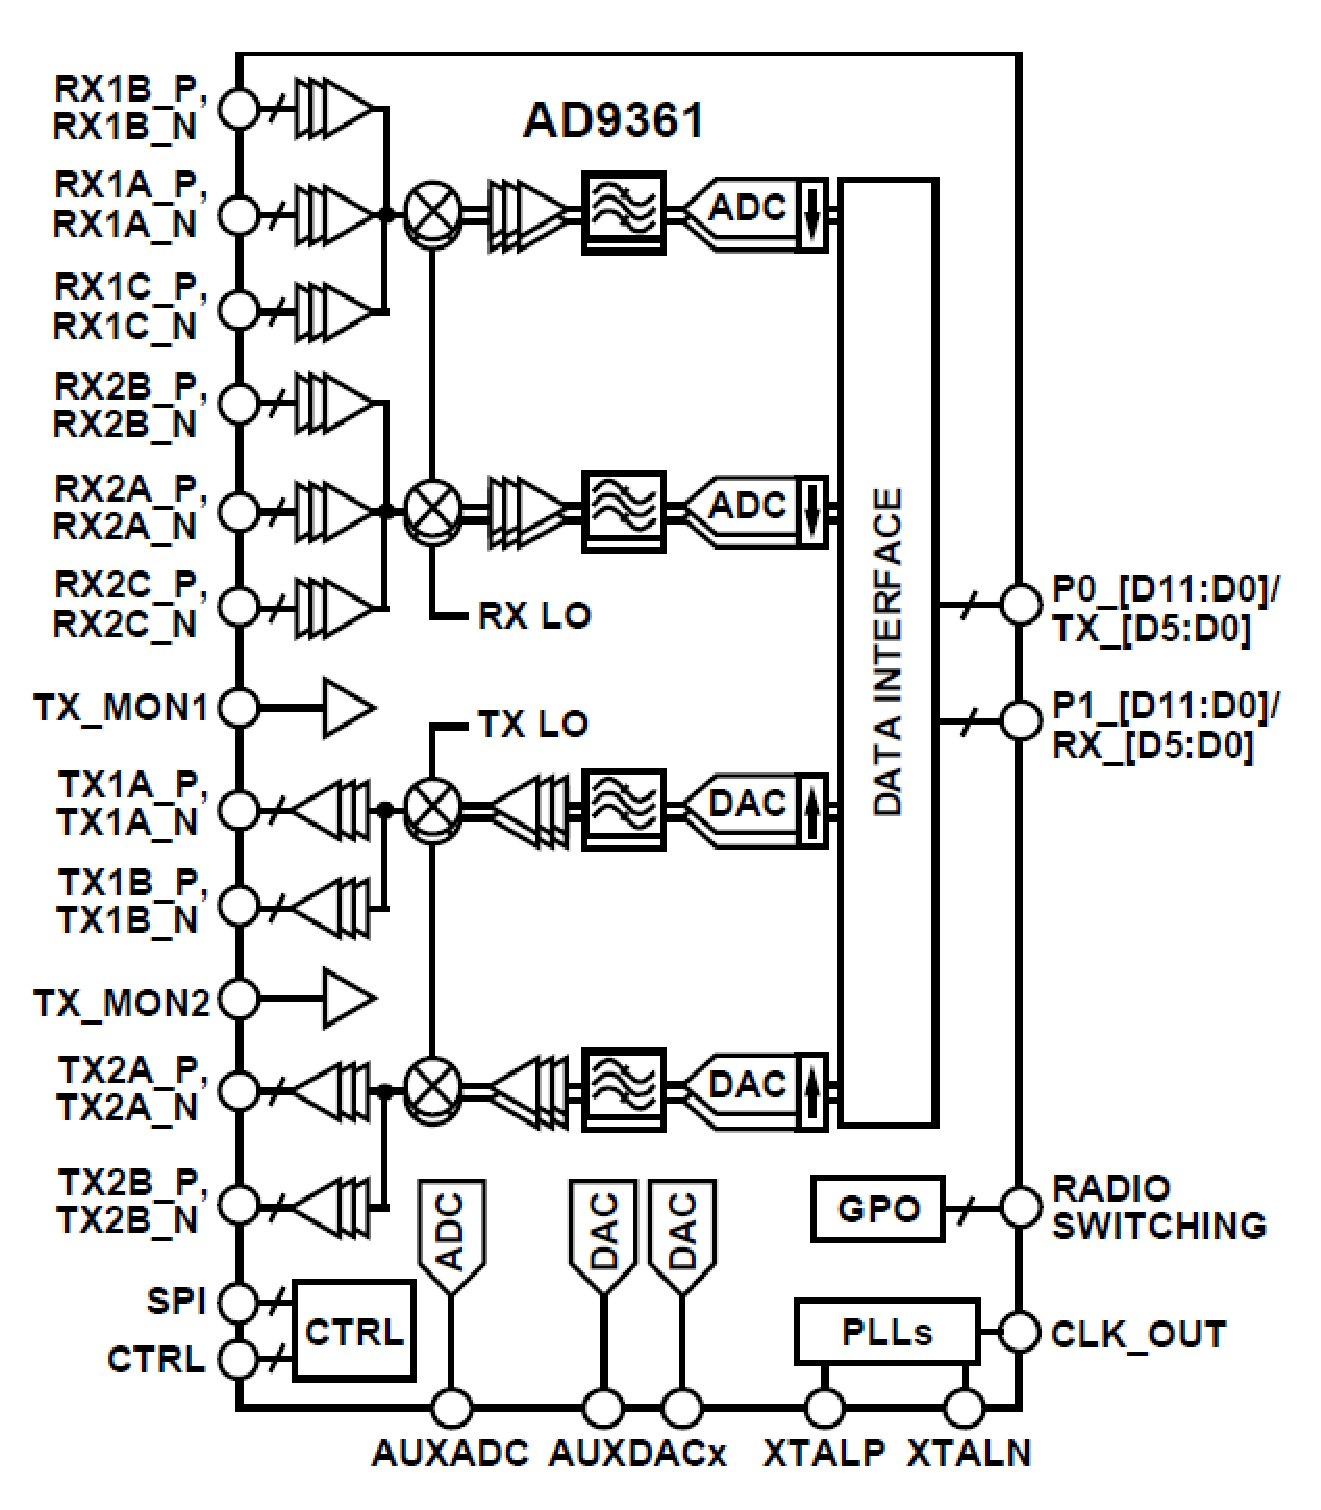
\includegraphics[width=0.65\textwidth]{./figures/ad9361_functional_diagram}
    \caption{ AD9361 Functional Block Diagram
    \label{fig:ad9361func}}
\end{figure}

\subsection{Receiver}

The receiver section has all the blocks necessary to receive analog RF signals and convert them to digital data which can be used by the BBP. there are two independently controlled channels that share same frequency synthesizer. This characteristic makes possible to the AD9361 to operate in MIMO systems.

Each channel has 3 inputs which can be multiplexed into the signal chain, making possible to use the AD9361 into systems with multiple antenna inputs. The Receiver is a direct conversion system that contains a Low noise amplifier (LNA) , followed by a matched in-phase and quadrature amplifier, mixers, and band shaping filters that down convert received signals to baseband for digitization. External LNAs can also be interfaced to the AD9361 allowing more flexibility in the design.
The receiver signal path passes downconverted signals (I and Q), which are schematically identical to each other,  to the baseband (BB) receiver section. The BB section is composed by two programmable low-pass filters, with programmable corner frequency for each filter, 12-bit ADC and four stages of decimating filters, each of the four decimation filters can be bypassed. 
The gain control is achieved by a preprogrammed gain index map, a lookup table for example, this map distributes gain in order to achieve optimal performance at each level. This optimal behavior can be achieved by enabling AGC, which can run in two modes, fast and slow gain control. This allow for the BBP to make gain adjustments as needed.
Each channel also contains independent RSSI measurement capability, DC offset tracking and all other circuitry needed for self-calibration.

The receiver ADC is a 12-bit sigma-delta ($\Sigma-\Delta$) ADC which allows adjustable sample rates. This ADC produces data streams from the received signals and such digitalized signals can be conditioned further by a series of decimation filters and a 128-tap FIR filter with additional decimation settings.
The sampling rate of each digital filter is adjustable through changes in the decimation factors to produce the needed data rate.

In short, the Receiver chain has:

\begin{itemize}
	\item LNA - Low noise Amplifier
	\item Matched in-phase amplifier;
	\item Quadrature Amplifier;
	\item Band Shaping Filters;
	\item Analog low pass filters;
	\item 12-bit DAC;
	\item 4 stages of decimation filters (128-tap FIR filters);
	\item Automatic gain Control;
\end{itemize}

\begin{figure}[htbp]
    \centering
    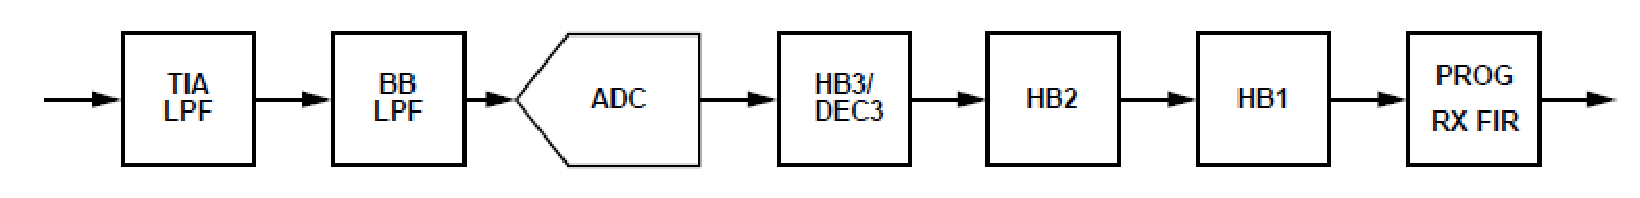
\includegraphics[width=0.65\textwidth]{./figures/rx_chain}
    \caption{ Receiver Signal Path
    \label{fig:rxchain}}
\end{figure}


\subsection{Transmitter}

Like the receiver section, the transmitter section contains two identical and independently controller channels, which share the same frequency synthesizer,  that provide all digital signal processing, mixed signal and RF blocks necessary to implement a direct conversion system from digital data to RF.
The Tx signal path receives from the BBP 12-bit 2s complement I-Q format data in the digital interface and each channel goes through a 128-tap FIR filter with interpolation options, which is fully programmable. Then the signal goes through a series of additional interpolation filters that manipulates the signal with additional filtering and data rate interpolation before reaching the 12-bit DAC, note that all these filtering and interpolation steps can be bypassed if desired.
Each 12-bit DAC has an adjustable sampling rate and its analog output passes through to low pass filters to remove any sampling artifacts before going to the RF mixer, these low pass filters corner frequencies can be programmable too. After all these filtering and analog conversion steps, the I and Q signals are recombined and modulated in the carrier frequency, which can be adjusted by changing the synthesizer frequency. These analog combined signals passes through additional analog filters for better band shaping and then it can be transmitted to the output amplifier. Each Transmitting channel provides wide attenuation adjustment range with fine granularity in order to optimize SNR.

\begin{figure}[htbp]
    \centering
    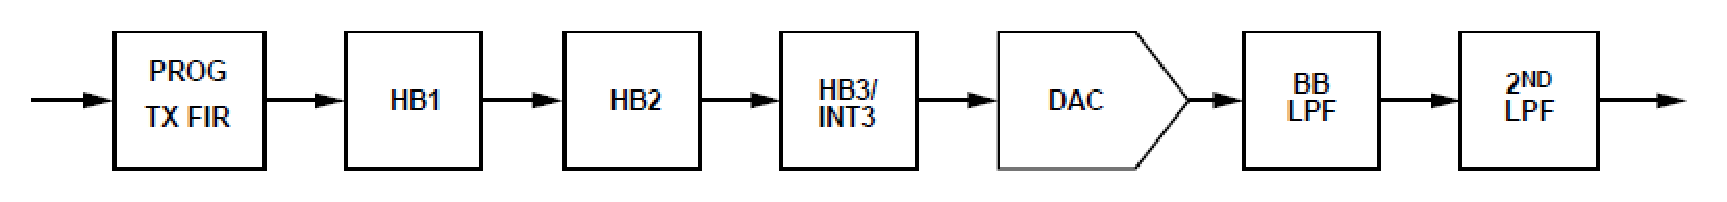
\includegraphics[width=0.65\textwidth]{./figures/tx_chain}
    \caption{ Transmitter Signal Path
    \label{fig:txchain}}
\end{figure}


Identical to the receiver chain, the transmitter chain has also built-in self-calibration circuitry into each transmitting channel providing an automatic real-time adjustment. The transmitter also provides a TX monitor block for each channel, this block monitors the transmission output and routes it back through an unused receiver channel to the BBP for signal monitoring, but these monitoring option is only available in TDD mode operation while the receiver is idle.

In short the transmission chain has:

\begin{itemize}
	\item 128-tap FIR filters;
	\item Interpolation Filters;
	\item 12-bit DAC;
	\item Analog Low-pass Filters;
	\item Additional band shaping analog filters;
	\item Attenuation adjustment;
	\item self-calibration circuits;
	\item Tx signal Monitor.
\end{itemize}

\begin{figure}[htbp]
    \centering
    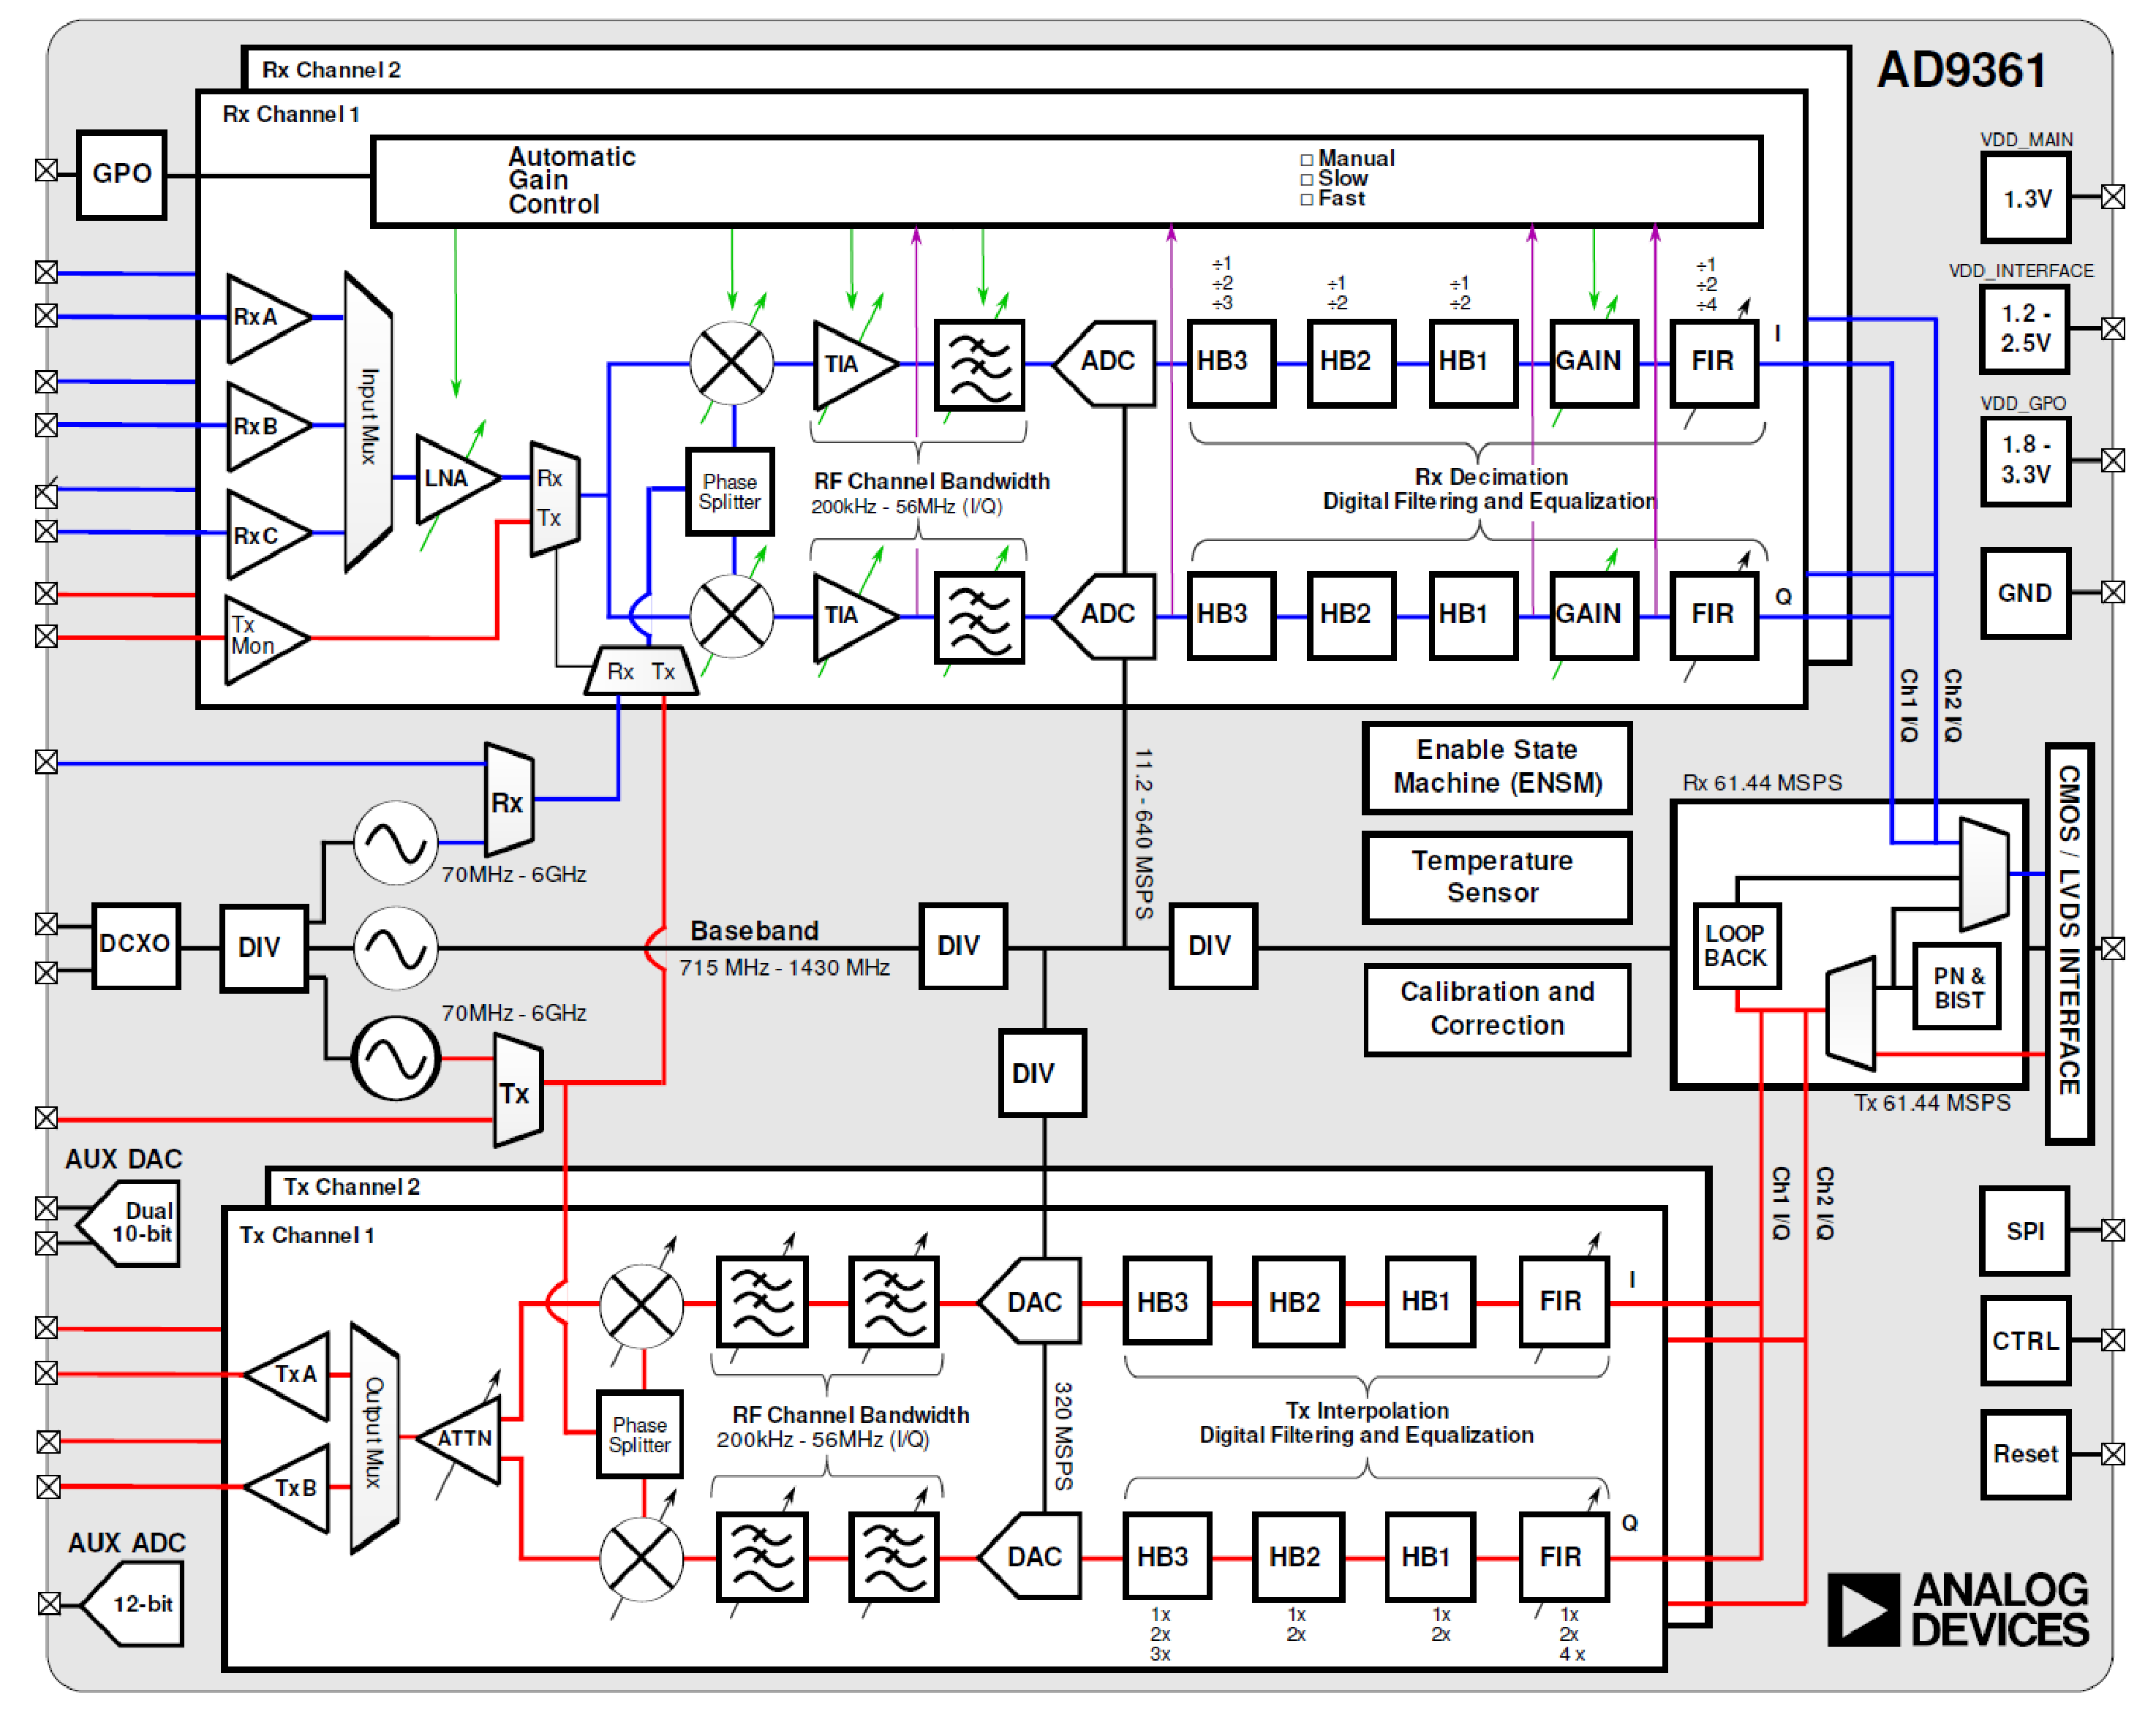
\includegraphics[width=0.65\textwidth]{./figures/ad9361_block_diagram}
    \caption{ AD9361 Block Diagram
    \label{fig:ad9361blk}}
\end{figure}

\subsection{Filtering}

In both receiver and transmitter there are:
\begin{description}
	\item[Receiver] \hfill \\
	\begin{itemize}
		\item Low pass filter : band shape to reduce adjacent-channel interference.
		\item Decimation Filter: up convert from the digital baseband rate (64.11MSPS max) to the actual ADC (640MSPS) rate.
	\end{itemize}
	\item[Transmitter] \hfill \\
\begin{itemize}
		\item Low pass filter : remove sampling artifacts
		\item Interpolation Filter : down convert from the digital baseband rate (64.11MSPS max) to the actual DAC (320MSPS) rate.
	\end{itemize}
\end{description}

In both digital and analog implementations these filters have impact the magnitude and the phase in passband, such behavior must be compensated in the system, and this compensation is usually done inside the 128-tap FIR filter. The FIR filter is not only used for low pass filter realization but also to compensate for magnitude and phase impacts created by the analog and digital half band filters in the desired baseband area. 

These filters depend in various other systems to work properly, such systems are sample rates, clock, data rates which sets the half band filters, and the desired RF bandwidth, which sets the analog filters. the process of loading a filter and after changing anything in the system will negatively affect the overall baseband performance. 

There is a filter too created by analog devices,which designs a low-pass filter and sets the FIR coefficients in order to ensure compensation for magnitude and phase changes in the analog or half band filters.

\subsection{Clocking}

%reescrever
The AD9361 has a series of internal PLL to generate and manipulate clock signals. There are fractional-n PLLs that generate the transmitter and receiver LO frequencies and there are the baseband PLL (BBPLL) used for the data converters, digital filters and I/O ports. All the frequency signals are generated using these PLLs clock outputs.

All the PLLs require a reference clock input and for this there is the digitally controlled oscillator (DXCO) function, which is an in-chip programmable and variable capacitor, such capacitor can tune the crystal frequency variance before entering the system, having a precision of +/- 6 ppm it results in a more accurate reference clock and can be used, if needed, for synchronization purposes. this function can also be used together with the on-chip temperature sensor to provide temperature compensation depending enviroment in which the chip will be used. For the reference clock there are two options:

\begin{description}
	\item[External Oscillator] \hfill \\
	In this option and external clock signal can be connected in the XTALP pin (Leaving the XTALP pin unconnected), this external clock frequency may vary from 10 MHz to 80 MHz. Such type of setup is needed when a wireless basestation (BTS) reference clock is locked to a master clock, and in such systems there is no or less need for clock synchronization.

	\item[Dedicated Crystal] \hfill \\
	In this option a dedicated crystal, with frequency varying from 19 MHz to 50 MHz, is connected in the XTALP and XTALN pins. This setup is usually used in wireless user equipment (UE), which do not need to be locked to a master clock but they do need to adjust periodically the LO frequency in order to maintain a connection with a BTS. The BTS periodically informs the UE of its frequency error relative to the BTS and the BBP can make adjustments to the reference clock and thus adjust the LO frequency if needed.

\end{description} 

\begin{figure}[htbp]
    \centering
    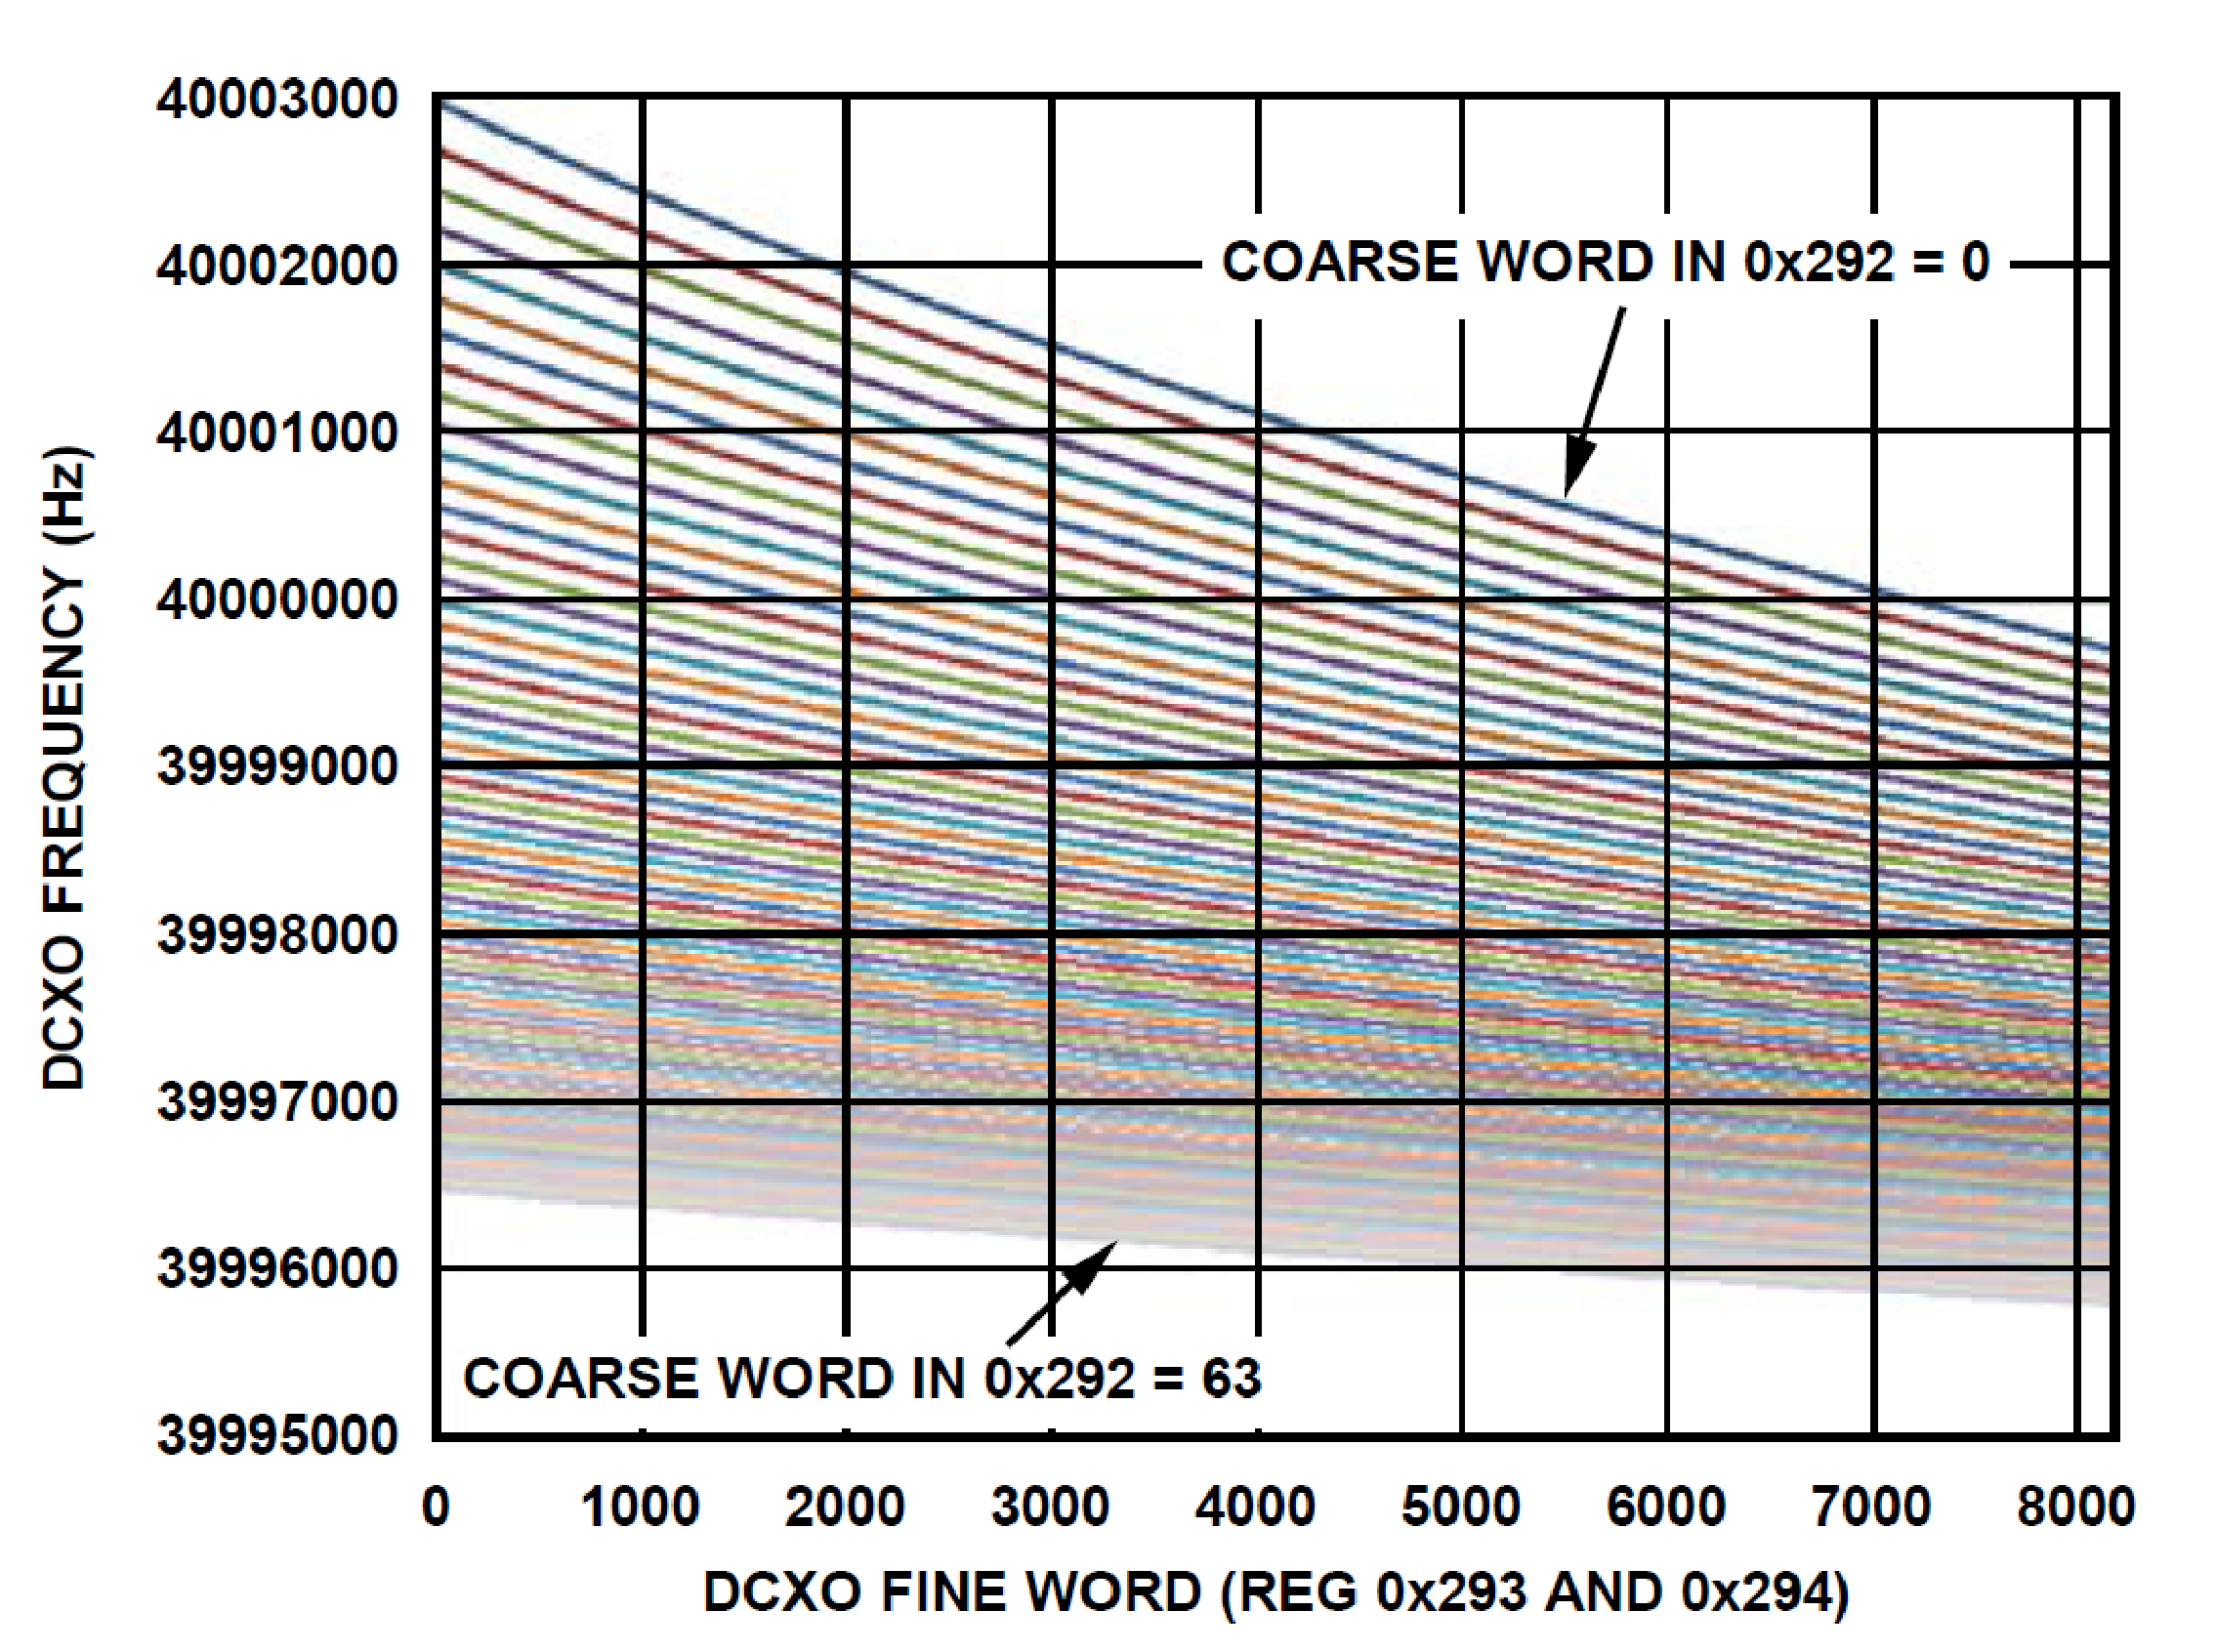
\includegraphics[width=0.65\textwidth]{./figures/dcxo_graph}
    \caption{ DCXO Behavior Graph
    \label{fig:pll}}
\end{figure}

\subsection{Synthesizers}

\begin{description}
	\item[RF PLLs] \hfill \\
	The AD9361 contains two identical synthesizers to generate the required LO signals for the RF signal path, one for the receiver and one for the transmitter. The PLL synthesizers are fractional-n PLLs with completely integrated VCOs and loop filters, requiring no other external components. In TDD operation mode, the synthesizers turn ON and OFF appropriate for the TX and RX frames, however in FDD TX PLL and RX PLL are activated at the same time.

	\item[BB PLL] \hfill \\
	The AD9361 contains also a baseband PLL synthesizer, which generate all the baseband related clock signals. The BBPLL feeds all the baseband related clock signals to ADC, DAC (Sampling Clock), DATA\_CLK signal and all data framing signals. This PLL has a frequency range from 700 Mhz to 1400 Mhz, and can be changed based on system requirements.

\end{description}

\begin{figure}[htbp]
    \centering
    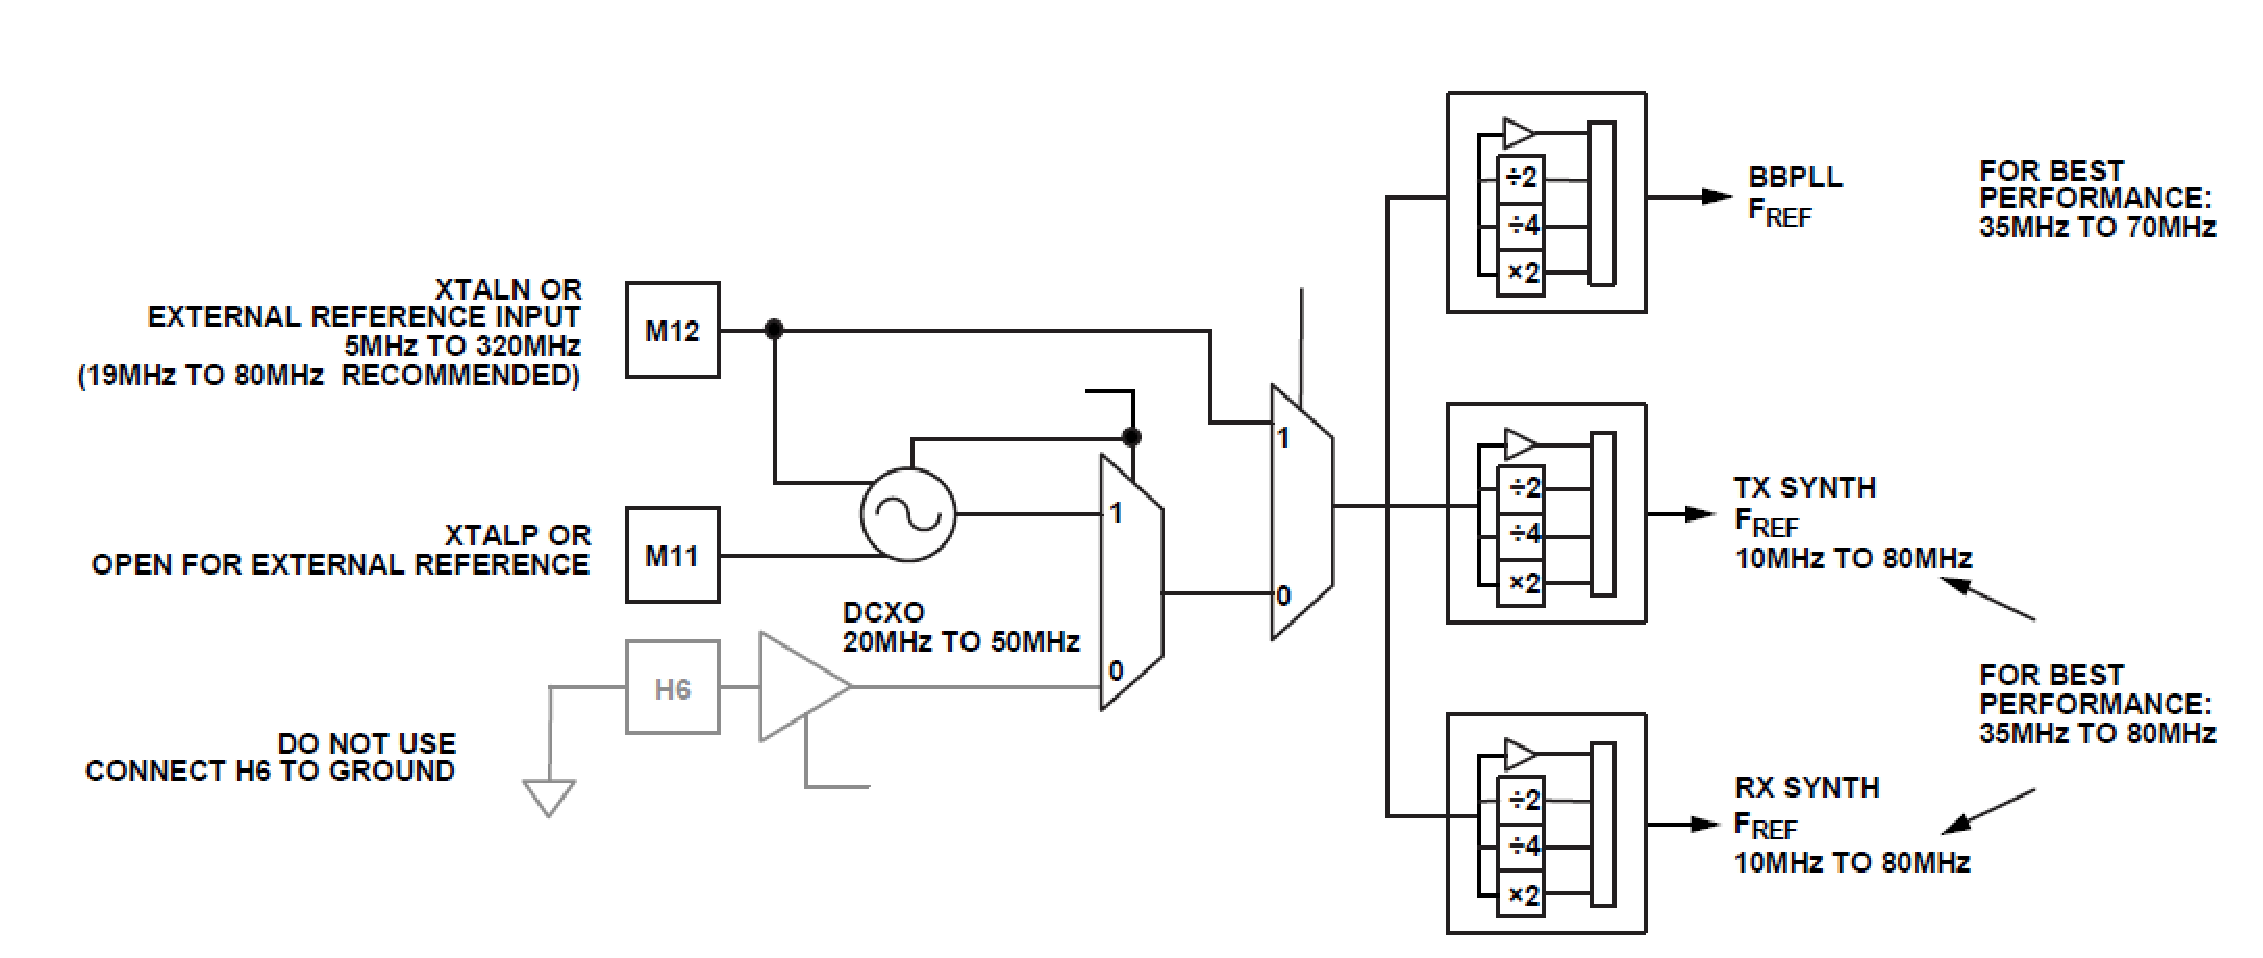
\includegraphics[width=0.65\textwidth]{./figures/pll_ref_block}
    \caption{ AD9361 PLL Reference Block Diagram
    \label{fig:pll}}
\end{figure}

\subsection{Digital Data Interface}

The AD9361 uses parallel data ports to transfer data between the device and the BBP. These data ports can be configured either single-ended CMOS format or LVDS format (used in this work). Both formats can be configured in multiple arrangements to adequate the system requirements for data transfer and connections. These arrangements can be of single port data bus, dual port data bus, single data rate, double data rate and other various combinations compatible with the device.\\
Bus transfers are controlled using hardware handshake signalling, these two ports can be operated in TDD (bidirectional) or FDD (full duplex) where half of the bits are used for transmitting and the other half is used for receiving. The interface can also be configured to use only one of the data ports ( usually used in applications that do not require high data rates or samples).\\
The communication between the BBP processor and the AD9361 rely on some signals to properly work, which are DATA\_CLK, FB\_CLK and RX\_FRAME, its operation is detailed below:

\begin{description}
	\item[DATA\_CLK Signal] \hfill \\
	RX sends the signal DATA\_CLK to the BBP, which can be used when receiving data. DATA\_CLK can be used to control data sampling time, which can be single data rate (data is captured on rising clock edge) or double data rate (data is captured on both rising and falling clock edges). This can be applied using single or dual data port.

	\item[FB\_CLK Signal] \hfill \\
	The FB\_CLK signal must have the same frequency and duty cycle as DATA\_CLK and like DATA\_CLK it is used as timing reference for the interface. FB\_CLK allows source synchronous with rising edge capture for burst control signals and can be used like DATA\_CLK for rising edge, single data rate mode or in both edge capture, double data rate mode for transmit signal bursts.

	\item[RF\_FRAME Signal] \hfill \\
	The RF\_FRAME signal is generated by the device whenever the receiver outputs valid data. RF\_FRAME has two modes:
	\begin{itemize}
		\item \textbf{Level Mode:} RF\_FRAME stays high as long as the data is valid.
		\item \textbf{Pulse Mode:} RF\_FRAME pulses with 30% duty cycle.
	\end{itemize}
	The BBP must provide a TX\_FRAME that indicates beginning of a valid data transmission with a rising edge. The TX\_FRAME operates similarly as the RF\_FRAME, on Level Mode or Pulse Mode.

\end{description}

\begin{figure}[htbp]
    \centering
    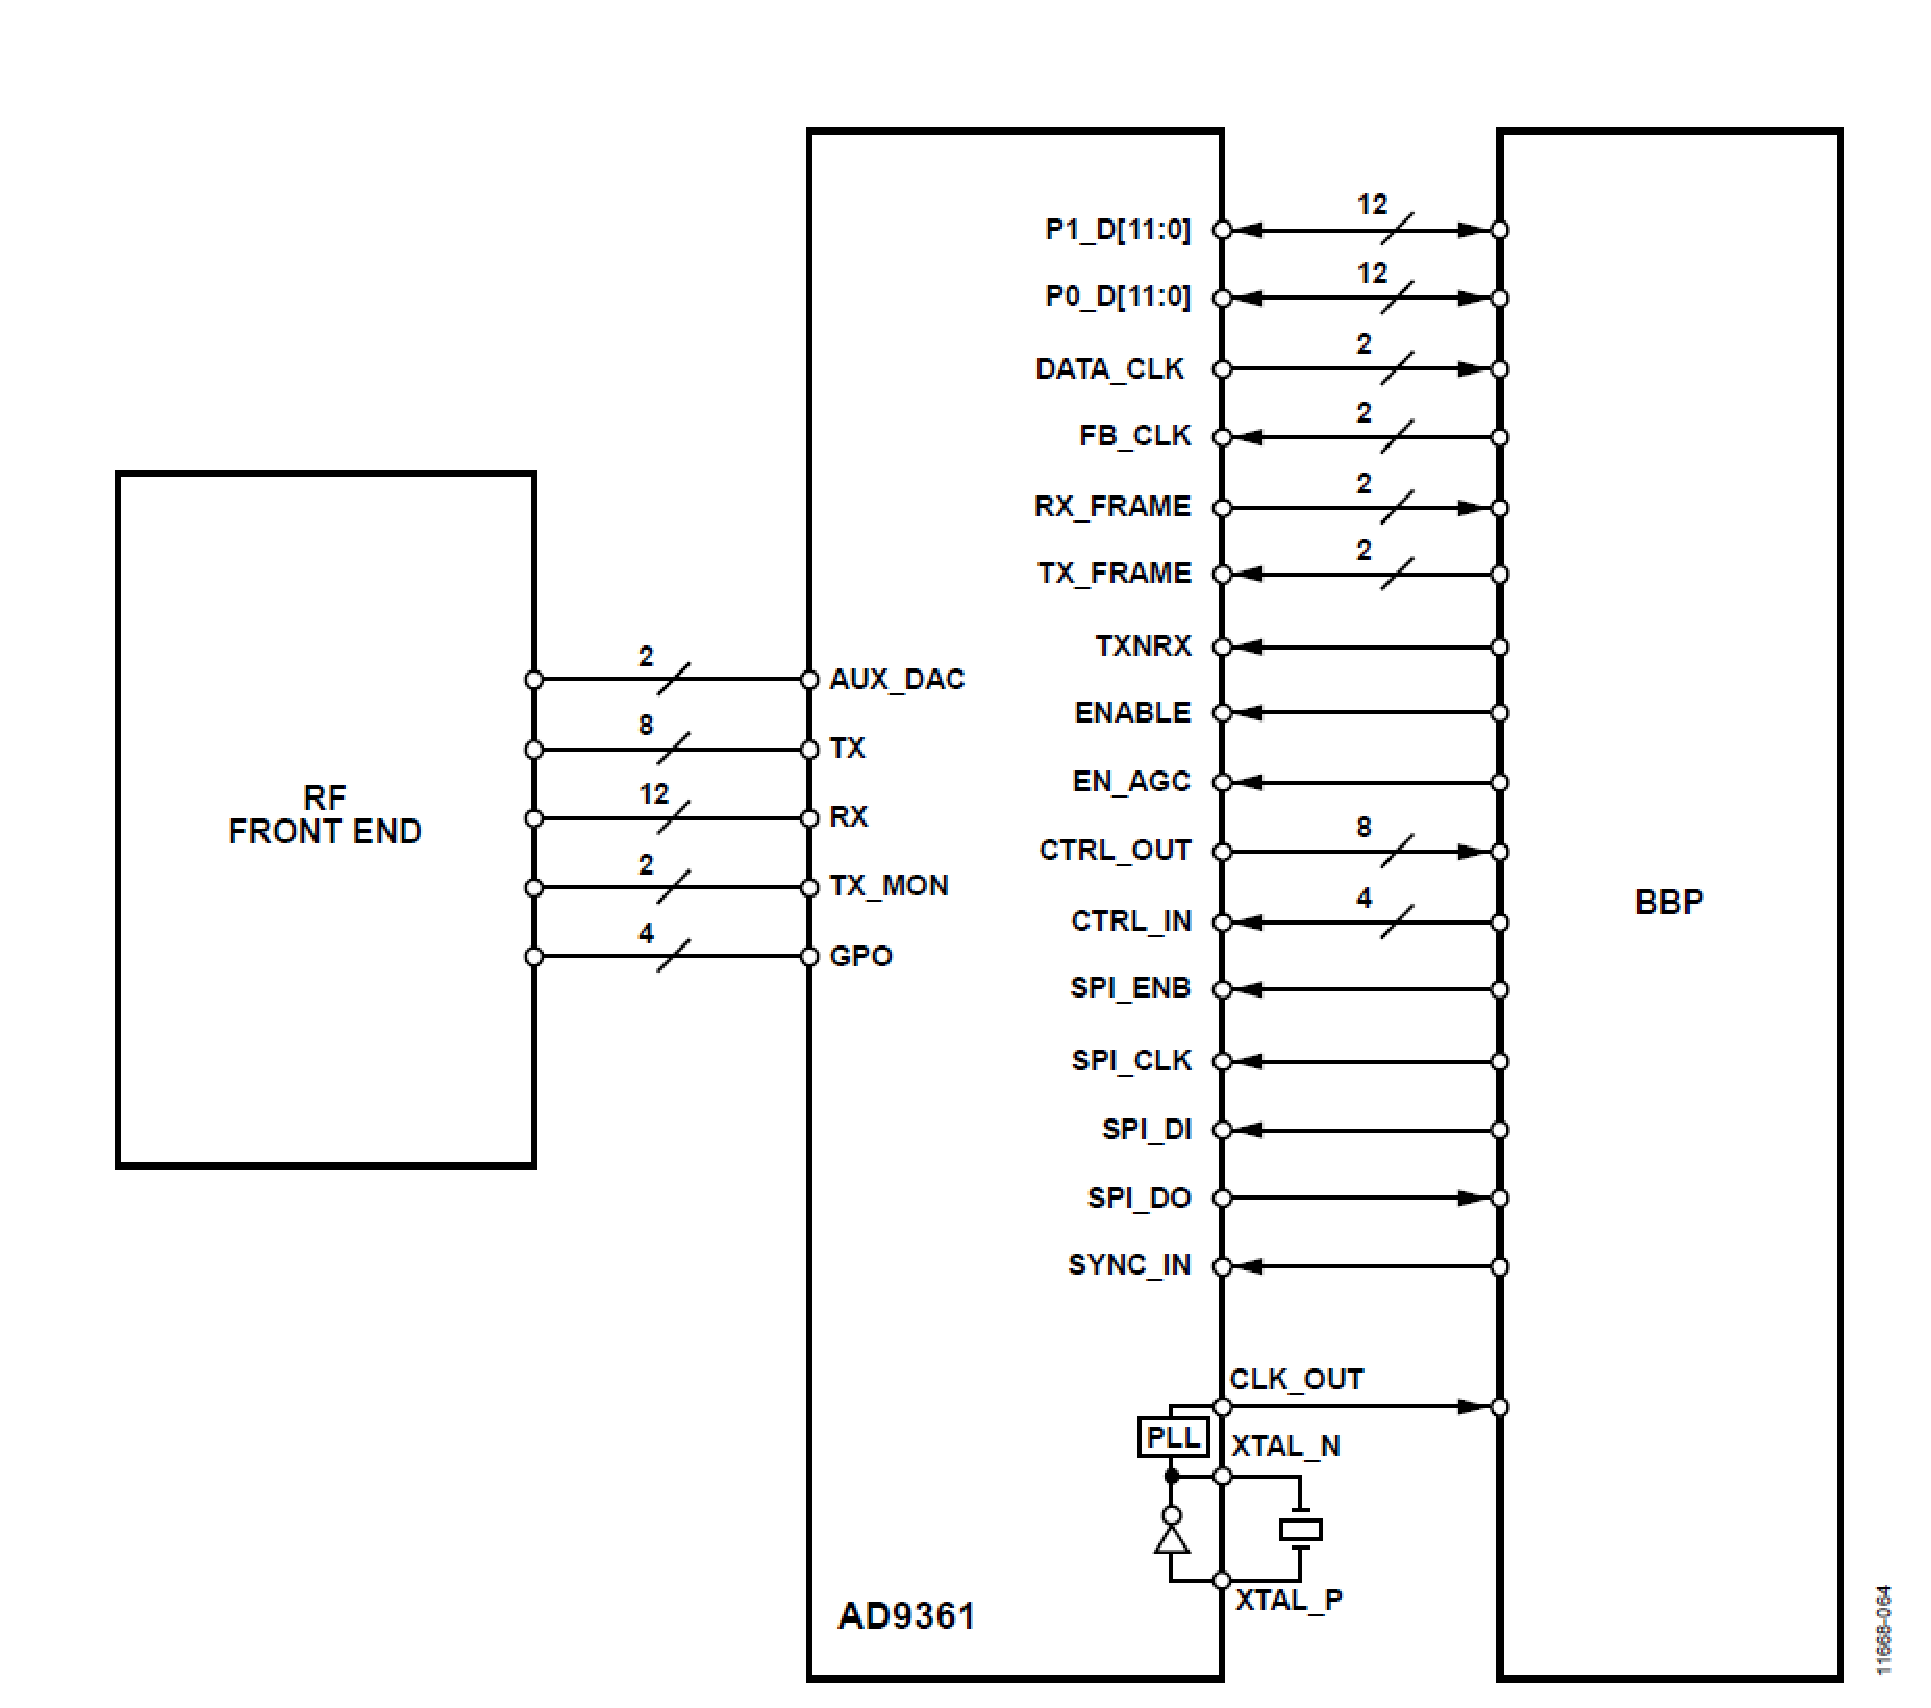
\includegraphics[width=0.65\textwidth]{./figures/ad9361_digital_interface}
    \caption{ AD9361 Digital Data Interface
    \label{fig:ad9361diginterface}}
\end{figure}


\subsection{Enable State Machine}

The AD9361 has an Enable State Machine (ENSM) which allows real-time control over the current state of the device. The device can be place in several states like:

\begin{itemize}
		\item \textbf{Wait:} Power save, synthesizers disabled.
		\item \textbf{Sleep:} Wait with all clocks and BBPLLs disabled.
		\item \textbf{TX:} TX chain enabled.
		\item \textbf{RX:} RX chain enabled.
		\item \textbf{FDD:}TX and RX chains enabled.
		\item \textbf{Alert:} Synthesizers enabled.
	\end{itemize}
	This ENSM can be controlled either by SPI or PIN (GPIO for example), where the SPI control mode is for a non real-time operation and the PIN control mode is for a much faster and real-time control.
	

\begin{description}
	\item[SPI Control Mode] \hfill \\
	In SPI control mode, the BBP writes registers asynchronously by using SPI protocol to access the addresses, and by writing these registers the state machine advances the current state to the next state. SPI communication is considerece asynchronous to the DATA\_CLK because the SPI\_CLK can be derived from another clock source, where BBP and the device does not share the same clock source. This control method is recommended when there is no need for a real-time control.

	\item[Pin Control Mode] \hfill \\
	In Pin control mode, there are pins dedicated to activate some states of the ENSM, like ENABLE pin and TXNRX pin, this mode allows a real-time control of the current state. This method is recommended in a system where the BBIC has extra pins to spare with the real-time control outputs, this 2-wire interface can control the state of the device.
	To advance the current state to the next state of the ENSM, the enable function of the ENABLE pin can be driven by either pulse or level,if the pulse is used the minimum width of the pulse needs to be equal as the FB\_CLK cycle.
	In FDD mode, the ENABLE and TXNRX pins can be remapped to be used as real-time control of the TX and RX data transfers. In this mode ENABLE enables or disables the receive signal and TXNRX enables or disables the transmit signal, using such mode  causes the ENSM to be removed from the system for data flow control and is replaced by these pins.

\end{description}

\begin{figure}[htbp]
    \centering
    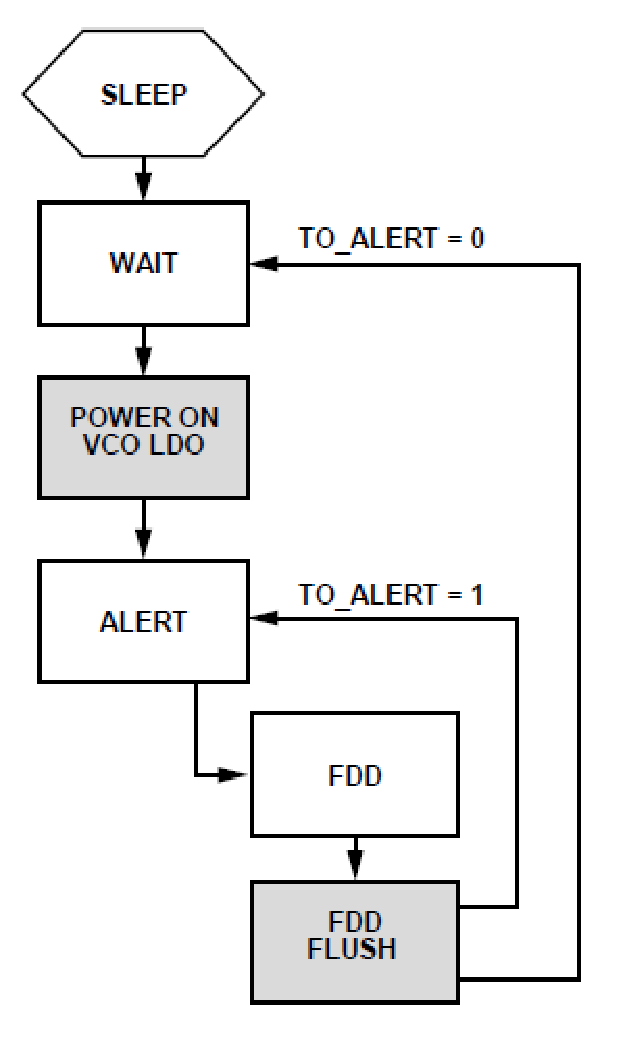
\includegraphics[width=0.65\textwidth]{./figures/fdd_ensm}
    \caption{ FDD Enable State Machine
    \label{fig:pll}}
\end{figure}

\begin{figure}[htbp]
    \centering
    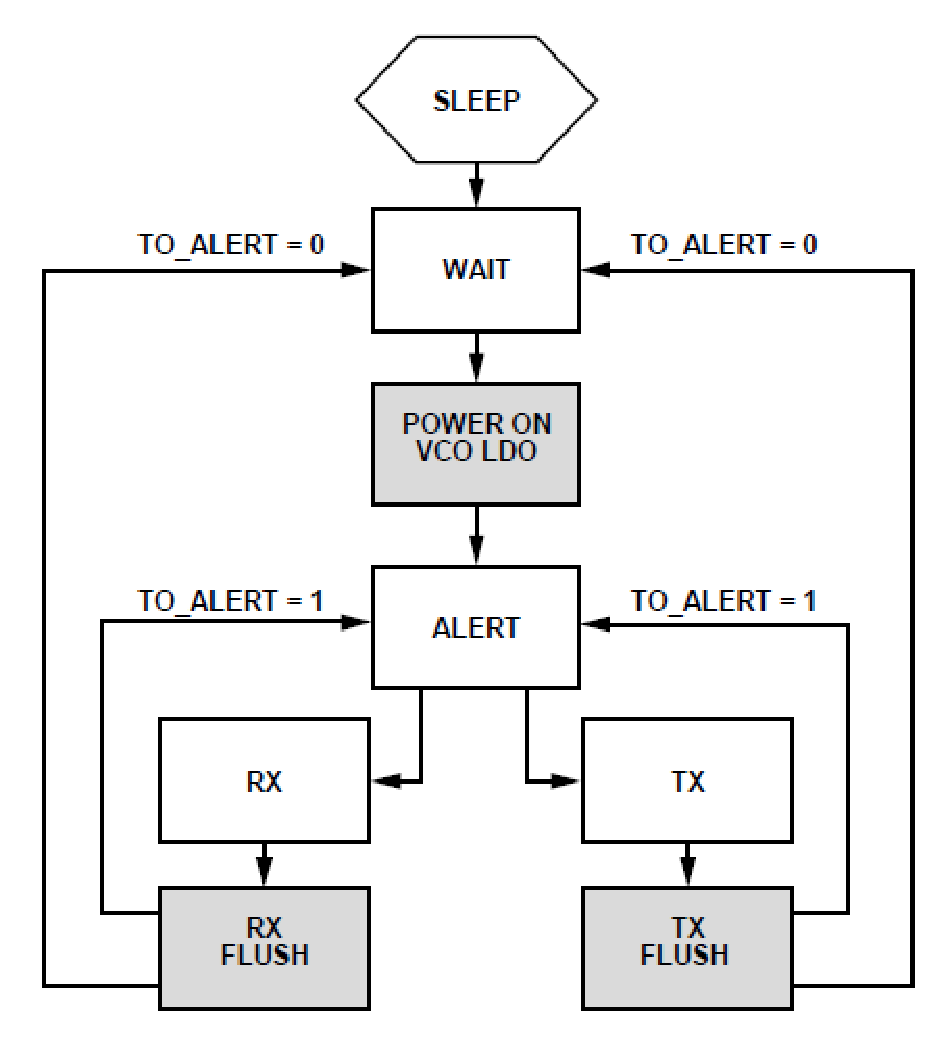
\includegraphics[width=0.65\textwidth]{./figures/tdd_ensm}
    \caption{ TDD Enable State Machine
    \label{fig:pll}}
\end{figure}


\subsection{SPI Interface}

The AD9361 uses a SPI interface for communication with the BBP. Throught SPI is possible to access all the device registers. The PSI interface can be configured as a 4-wire interface with dedicated transmit and receive pins, duplex, or as 3-wire interface with bidirectional data port. 
Write commands have a 24-bit format where the first six bits are for setting the bus direction and number of bytes to transfer, the next 10 bits set the address where the data is to be written and the final eight bits are the data to be transferred to the specific register address (MSB to LSB), a LSB-first format is also supported.
Read commands follow a similar format, the difference is that the first 16 bits are transferred on the SPI\_DI pin and the final eight are read from the AD9361, either using SPI\_DO (4-wire interface) or SPI\_DI (3-wire interface).

\subsection{Auxiliary Converters}

\begin{description}

	\item[AUXADC] \hfill \\
	The AD(361 contains an auxiliary ADC that can be used to monitor some system functions such as temperature or power output, it is a 12-bit converter and has an input range of 0V to 1.25V. The SPI can read the last value latched at the output of the ADC when it is enabled for use, there is also a multiplexer that permits to select between AUXADC and built-in temperature sensor.

	\item[AUXDAC1 and AUXDAC2] \hfill \\
	The AD(361 also has two identical auxiliary DACs which can be used to provide power amplifier (PA) bias or other system functionality. Both the DACs are 10-bit wide and have an output range of 0.5 V to 0.3V and have a current drive of 10mA. The DACs can be directly controlled by the ENSM.

\end{description}

\subsection{Applications}


\section{FMCommS2}

FMCommS2 is basically evaluation board for the AD9361 that has a FPGA Mezzanine Card (FMC) connector for interfacing with the BBP (Usually FPGA). The FMComms2 has 5 SMA connectors, 2 for Rx, 2 for Tx and one for external reference clock input. The FMComms2 provides a 2x2 RF configuration, extended from the AD9361, and has  a narrow tuning range balun, which is performance optimized for 2.4GHz.
The FMComms2 is a transceiver intended for use in RF applications such 3G or 4G BTS or SDR. Its programmability and wideband capability make it ideal for broad range of transceiver applications and make it very attractive for the new C-RAN paradigm.

\begin{figure}[htbp]
    \centering
    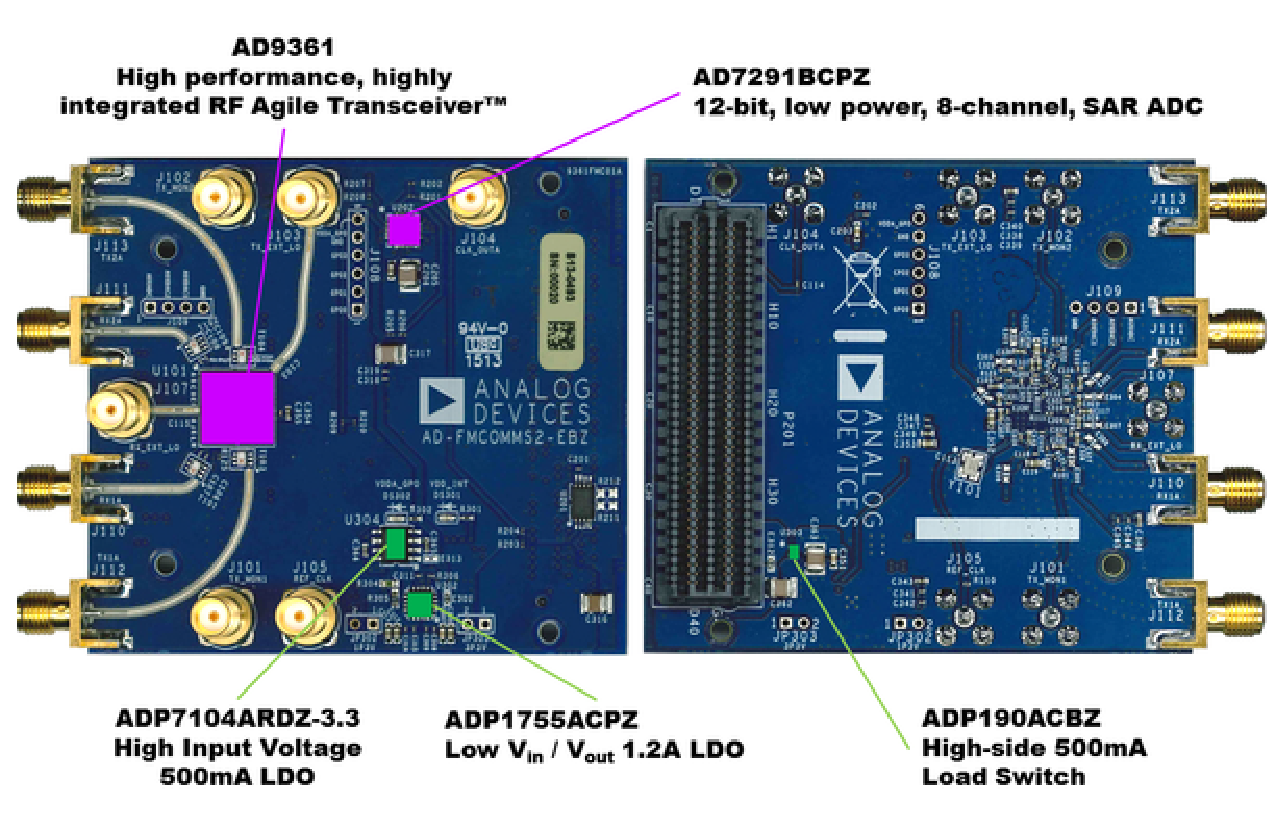
\includegraphics[width=0.65\textwidth]{./figures/fmcomms2_pic}
    \caption{ FMComms2 and its components
    \label{fig:fmcomm}}
\end{figure}


\subsection{Functional Overview}

The Block diagram show that there are 4 main functional partitions - receiver path, transmit path, clocking and power supply. Since the FMComms2 incorporates and extends the basic functionalities of the AD9361, thus the data path is fully integrated into the AD9361.

\begin{figure}[htbp]
    \centering
    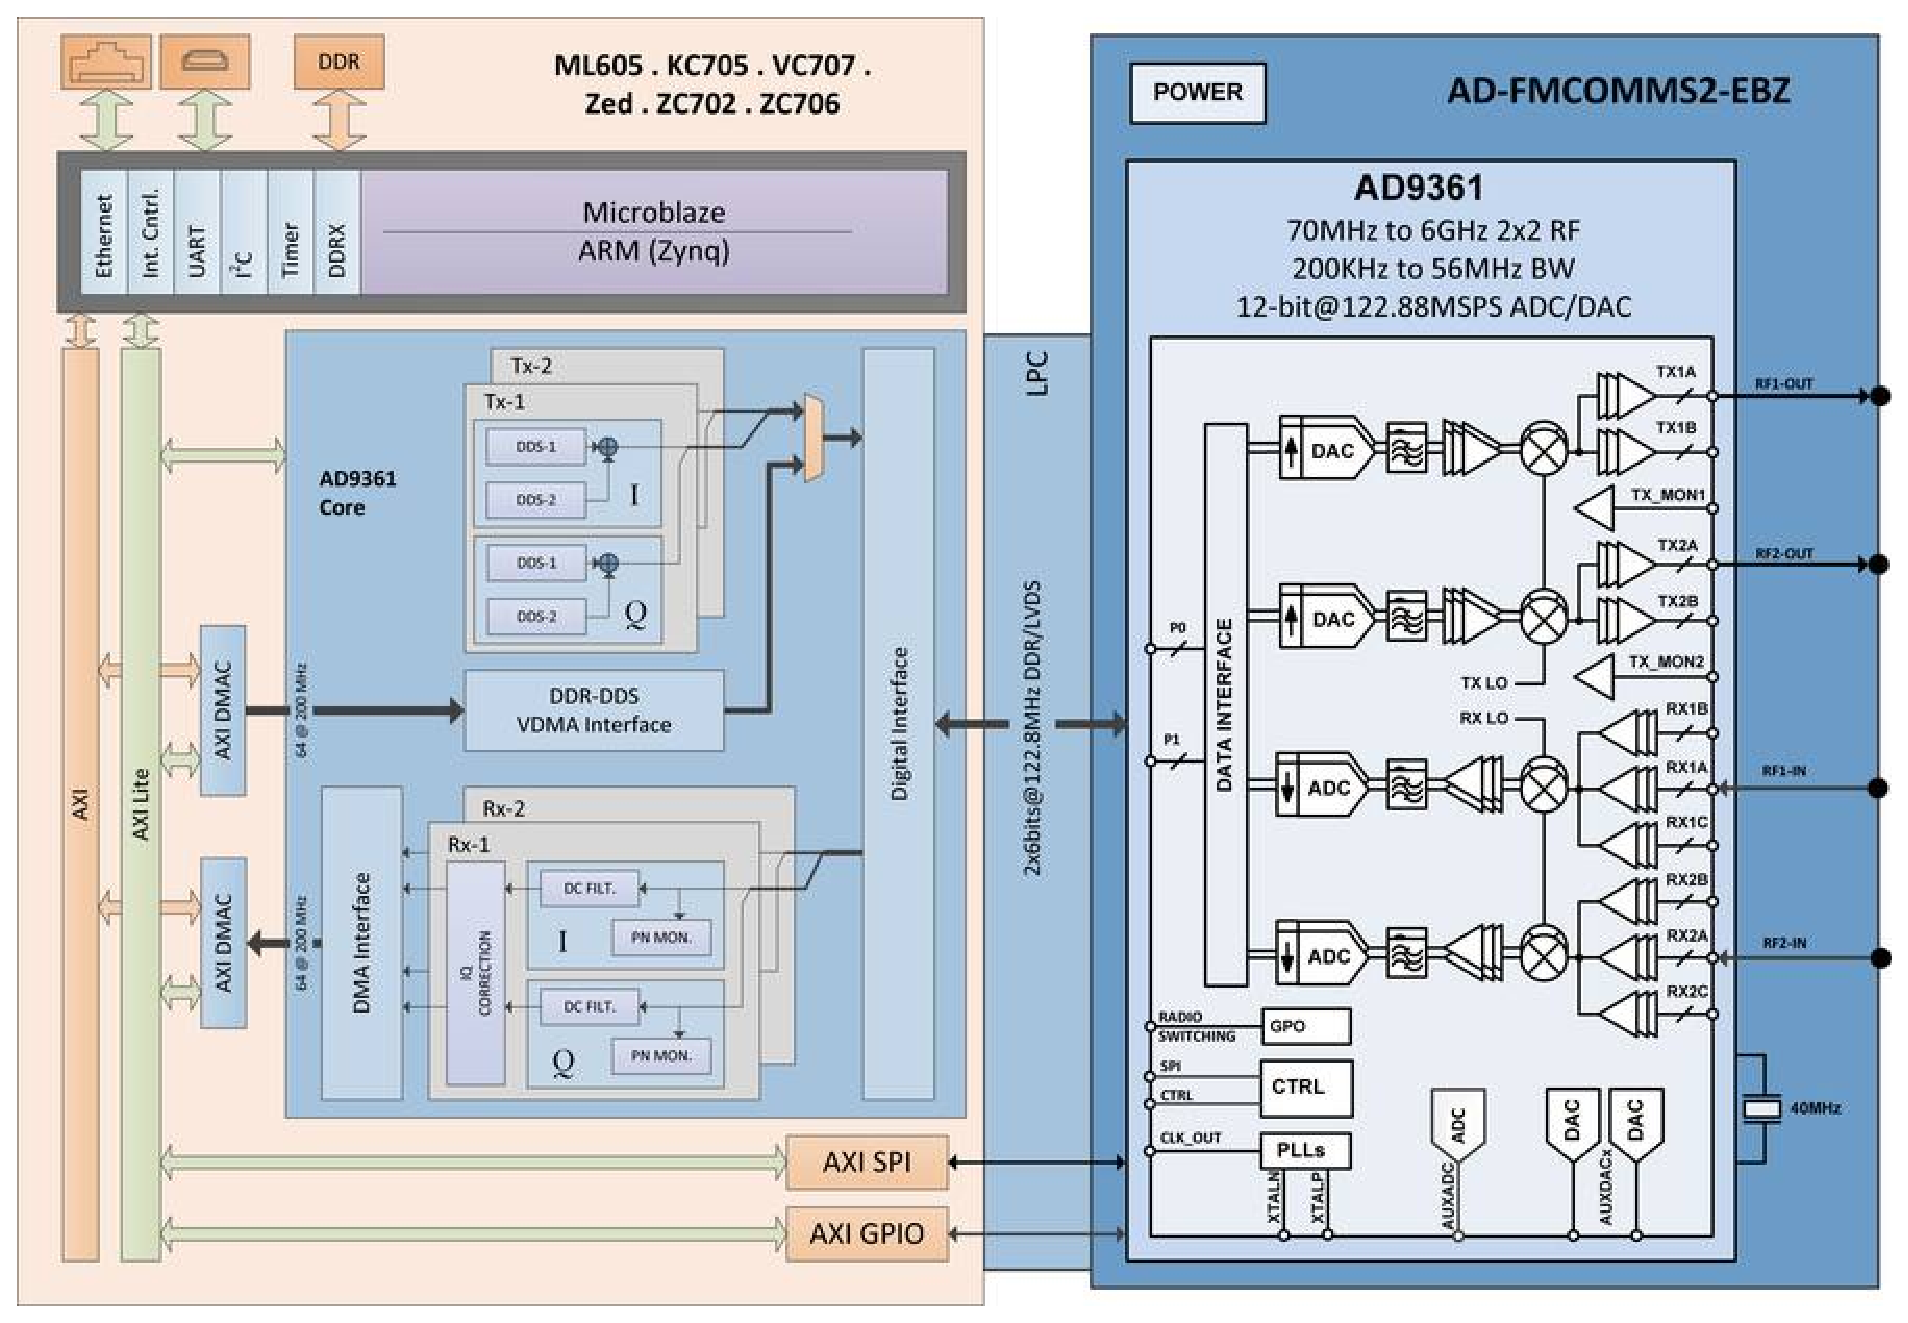
\includegraphics[width=0.65\textwidth]{./figures/fmcomms2_bd}
    \caption{ FMComms2 and FPGA Block Diagram
    \label{fig:fmcommbd}}
\end{figure}



\begin{description}
	\item[Receive] \hfill \\
	\begin{itemize}
		\item Support up to 2 direct conversion RF receiver channels.
		\item Fully integrated frequency synthesizers (including loop filter).
		\item Data path consists in LNA, Demodulator, LPF, ADC and digital filters.
		\item \textit{AGC:} quadrature calibration and DC offset calibration.
		\item \textit{NF:} 2.5 dB at 1Ghz.
		\item \textit{ADC:} Continuous time sigma-delta ( $\Sigma - \Delta$), 640 MSPS.
		\item \textit{Digital FIlter:} 128 COmplex taps with decimation between 2 and 48.
		\item \textit{Gain:} 1dB step size, 80 dB analog Range, 30 db digital range (post ADC scaling).
		\item On-chip sensor for temperature corrected RSSI.
	\end{itemize}

	\item[Transmit] \hfill \\
\begin{itemize}
		\item Supports up to 2 direct conversion RF transmit channels.
		\item Fully integrated frequency synthesizers (including loop filter).
\item Data path consists of digital filters, DAC and modulators.
		\item \textit{Digital FIlter:} 128 complex taps with interpolation between 2 and 48.
		\item \textit{Gain:} 0.5 dB step size, 86 dB range.
		\item \textit{ADC:} 340 MSPS.
	\end{itemize}

	\item[Clocking] \hfill \\
		The FMComms2 board has a integrated crystal oscillator of 40 Mhz and has a SMA input for external clock input.

	\item[Control/Monitor] \hfill \\
		The board allows real time control and monitoring via dedicated pins, such pins functionality are programmable. The control and monitor programming configuration is specified in the ad9361 section \cite{sec:ad9361}.

\end{description}

\section{Basic Mathematical Background}

\subsection{Complex Modulation}

\begin{eqnarray}
	I = sin(\omega \times t)\\
	Q = cos(\omega \times t)
\end{eqnarray}

\begin{equation}
	cos(\omega \times t) = sin(\frac{\pi}{2} - (\omega \times t))
\end{equation}

then:

\begin{eqnarray}
	I = sin(\omega \times t)\\
	Q = sin(\frac{\pi}{2} - (\omega \times t))
\end{eqnarray}

These are the two signals coming out of the DAC, two sine waves, phase offset from each other, wich is called IQ.

\subsection{Basic Modulation Mathematics}

Start to modulating signal from a amplitude perspective:

\begin{eqnarray}
LO_I = A_x cos(k)\\
LO_Q = B_x sin(k)
\end{eqnarray}

We still have the carrier:

\begin{equation}
LO_I = cos(\omega) ; LO_Q = sin(\omega)
\end{equation}

Will result:

\begin{eqnarray}
LO_I \times I = A_x cos(k) \times sin(\omega)\\
LO_Q \times I = B_x sin(k) \times cos(\omega)
\end{eqnarray}


That gives the output:

\begin{equation}
x(t)=A_x cos(k)\times sin(\omega)+ B_x sin(k)\times cos(\omega)
\end{equation}

This does not match with any trigonometrical identities and it is easier to use Euler\'s formula:

\begin{eqnarray}
sin(x)=(\frac{1}{2}e^{-jx} - \frac{1}{2}e^{jx})\\
cos(x)=(\frac{1}{2}e^{-jx} + \frac{1}{2}e^{jx})
\end{eqnarray}

Therefore:

\begin{equation}
x(t)=A_x (\frac{1}{2}e^{-jk} + \frac{1}{2}e^{jk})\times (\frac{1}{2}e^{-j\omega} - \frac{1}{2}e^{j\omega})+ B_x (\frac{1}{2}e^{-jk} - \frac{1}{2}e^{jk})\times (\frac{1}{2}e^{-j\omega} + \frac{1}{2}e^{j\omega})
\end{equation}

\begin{equation}
x(t)=\frac{A}{2} (e^{-jk} + e^{jk})\times (e^{-j\omega} - e^{j\omega})+ \frac{B}{2} (e^{-jk} - e^{jk})\times (e^{-j\omega} + e^{j\omega})
\end{equation}

If we expand we get:

\begin{equation}
x(t)=\frac{1}{2} ((Ae^{-jk-j\omega} + Ae^{jk-j\omega} - Ae^{-jk+j\omega} - Ae^{jk+j\omega}) + (Be^{-jk-j\omega} - Be^{jk-j\omega} - Be^{-jk+j\omega} + Be^{jk+j\omega}))
\end{equation}


And then:

\begin{equation}
x(t)=\frac{1}{2} ((A+B)e^{-jk-j\omega} + (A-B)e^{jk-j\omega} - (A-B)e^{-jk+j\omega} - (A+B)e^{jk+j\omega})
\end{equation}

It is possible to rearrange as:

\begin{equation}
x(t)=\frac{1}{2} \times ((A+B)(e^{-jk-j\omega} - e^{jk+j\omega}) + (A-B)(e^{jk-j\omega} - e^{-jk+j\omega}))
\end{equation}

And then:

\begin{equation}
x(t)=(\frac{A+B}{2} )(sin(k+\omega)) + (\frac{A-B}{2} )(sin(k-\omega))
\end{equation}

If this due to amplitude mismatch, this creates an image on the other side of the local oscillator.





\chapter{FPGA}
\section{ML605 - Virtex6}
\section{VC707 - Virtex7}

\chapter{Setup Description}


\section{Overview}

\section{Integration between FPGA and FMComms2}


\part{Final Results}
\chapter{Results}

\section{Preliminary Tests}

\section{Transmission Tests}



\part{Conclusion and Future Work}
\chapter{Conclusion}
\label{chap:conclusion}

\section{Conclusion}
\label{sec:conclusion}

The development of this setup was meant to be general and be used in both
research and academic environments. The process of implementing this setup went
through a myriad of fields in telecommunications and embedded systems, such as
communication protocols, embedded programming, electronics and many others,
being this setup a testbed for more complex processes inside the LTE band saves
a lot of time in development. \\

The FMComms2 board allows real-time and scalable change in parameters by
software or hardware signals, and it re-calibrates and reconfigures itself if
needed so, which makes a very good transceiver board to be used in a C-RAN
environment.\\

This setup was extensively documented and can be used in digital communication
classes to show how a real radio frontend system is made, of course there is
much to improve, there is no dynamic clock synchronization between the FPGA and
the FMComms2, there is no communication protocol between the FPGA (BBP) and the
external world other than the FMComms2 such things are necessary to have a real
frontend but were outside the scope of this project which was just to evaluate a
setup for a scalable and dynamically configurable frontend.\\

Although the FMComms2 and the FPGA operates on different clocks, thus no real
synchronization was implemented, this setup has the minimal capability of
transmitting and receiving signals and reconfigure itself on real-time, the main
goal of this work was reached, however there is much to explore with these tools
and devices.

\section{Future Works}
\label{sec:futurew}

Having finished this part of the work a natural sequel would be implementing
Ethernet connection driver in the FPGA, making it possible to receive data from
Ethernet and hand this to the transceiver board following the schematic on
figure \ref{fig:setupeth} idea. This would be a challenge because there is a lot
of things to consider, but the most problematic of them all is synchronization,
the clock in which everything inside the FPGA works is different from the AD9361
clock not only in frequency but in phase, this can bring a lot of problems,
however there is the possibility of feeding FMComms2 with an external clock
which would increase its performance.\\

With Ethernet it would be possible to generate the modulated samples and send
them trough air, just like Gnuradio + USRP and thus demodulate the received back
samples in the PC, however there is another possibility, modulation and
demodulation blocks implemented in the FPGA logic, thus much faster than the PC
ones and with partial reconfiguration there is the advantage of loading various
schemes of modulation/demodulation in the FPGA, implementing thus a very good
SDR. The Ethernet connection, is also very interesting for C-RAN
environment, because Ethernet is cheap and easy to implement.\\

\begin{figure}[htbp]
    \centering
    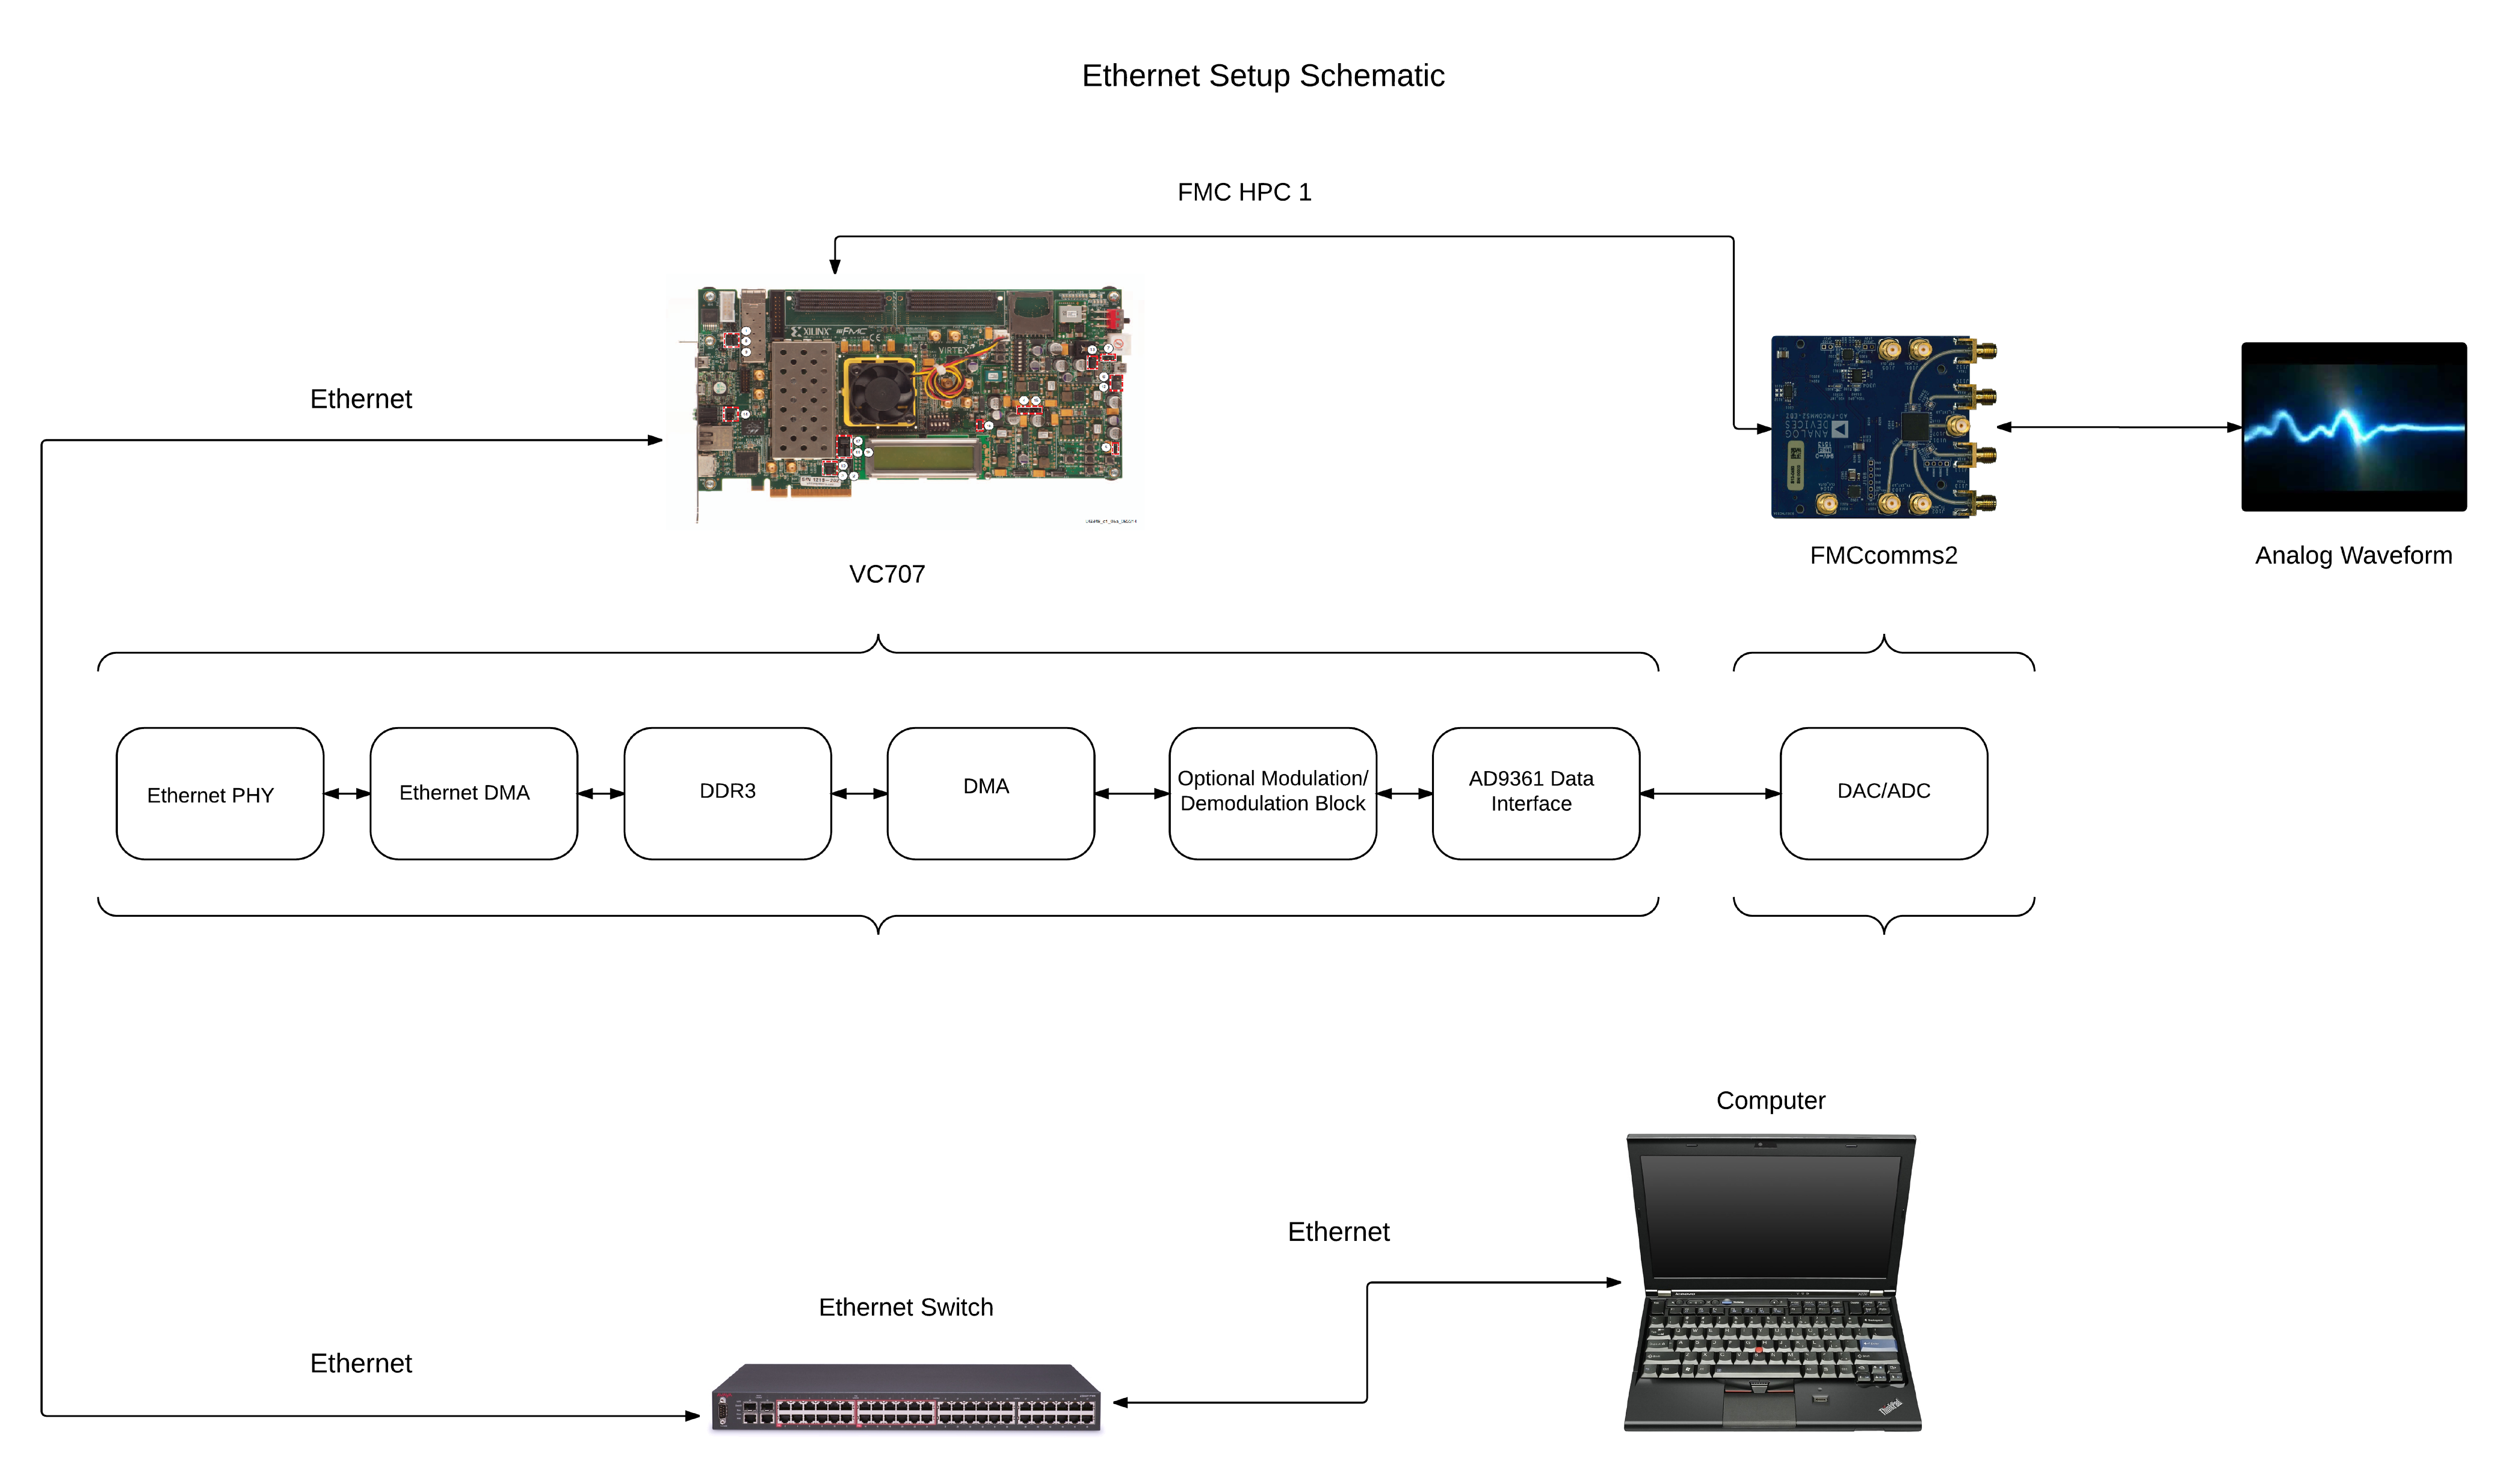
\includegraphics[width=0.65\textwidth]{./figures/eth_setup}
    \caption{ Setup Enhanced with Ethernet Connection
    \label{fig:setupeth}}
\end{figure}


%%%%%%%%%%%%%%%%%%%%%%%%%%%%%%%%%%`
%   Referencias bibliograficas   %
%%%%%%%%%%%%%%%%%%%%%%%%%%%%%%%%%%

\renewcommand\bibname{References}
%\bibliographystyle{../../../public/ABNT-20020112}
%\bibliographystyle{../public/IEEEtran}
%\bibliographystyle{../../../Public/IEEEtran_pt}
\bibliographystyle{abnt}
\bibliography{references}

%temorary tag just while there is no \citation
%eliminates no \citation error
\nocite{*}

\clearpage

%%%%%%%%%%%%%%%%%%%%%
%   Apêndices    %
%%%%%%%%%%%%%%%%%%%%%

\appendix
\chapter{PLL}
\chapter{FPGA Design Flow}
\chapter{AD9361 NO-OS Driver}


%%%%%%%%%%%%%%%%%%%%%
%   Página em branco    %
%%%%%%%%%%%%%%%%%%%%%

\newpage
\thispagestyle{empty}
\mbox{}

%% -- Termino do TCC
\end{document}
